   \documentclass[a4paper, 12pt]{article}
   \usepackage[utf8]{inputenc}
   \usepackage[french]{babel}
   \usepackage[T1]{fontenc}
   \usepackage[left=2.5cm,right=2cm,top=2cm,bottom=2.5cm]{geometry}
   \usepackage{xspace}
   \usepackage{marvosym}
   \usepackage{pdfpages}
   \usepackage{pdflscape}
   \usepackage{pgf, tikz}
\tikzstyle{n}=[rounded corners=3pt,fill=gray!35, minimum width, text centered] 
\tikzstyle{edge from parent}=[thick,draw]
   \usepackage{pgfplots}
   \usepackage{pgfplotstable}
   \usepgfplotslibrary{dateplot}
   \usetikzlibrary{pgfplots.dateplot}
   \usetikzlibrary{plotmarks}
   \tikzset{every mark/.append style={scale=0.5}}
   \usetikzlibrary{arrows, shapes, positioning}
   \usepackage{tikz-qtree}
   \usetikzlibrary{mindmap}
   \usepackage{lmodern}
   \usepackage[hyphens]{url} 
   \usepackage[toc,page,title]{appendix}
\renewcommand{\appendixtocname}{Annexes}
\renewcommand{\appendixpagename}{Annexes}

   \usepackage{gensymb}
   \usepackage{fancyhdr}
   \pagestyle{fancy}
\lhead{}
\chead{}
\rhead{} 
\lfoot{}
\cfoot{2018-2020}
\rfoot{\thepage}
\renewcommand{\headrulewidth}{0.4pt} \renewcommand{\footrulewidth}{0.4pt}
  
   \usepackage[pdfauthor={{Prénom Nom}}, pdftitle={{Titre document}}, pdfstartview=Fit, pdfpagelayout=SinglePage, pdfnewwindow=true, bookmarksnumbered=false, breaklinks, colorlinks, linkcolor=gray, urlcolor=black, citecolor=cyan, linktoc=all]{hyperref}
\newlength\epaisLigne \newcommand\Ghline{\noalign{\global\epaisLigne\arraywidth\globa
\arrayrulewidth 1pt}\hline \noalign{\global\arrayrulewidth\epaisLigne}}

   \usepackage{multicol}
   \usepackage{graphicx}
   \usepackage{array} 
   \usepackage{tabularx}
   \usepackage{ltablex}
   \usepackage{arydshln} 
   \renewcommand{\arraystretch}{1.25}
   
   \begin{document}
 
\begin{titlepage}

\newcommand{\HRule}{\rule{\linewidth}{0.5mm}}

\center 
 
\huge\textsc{\Large Association Ouvrière des Compagnons du Devoir et du tour de France}\\

 \begin{figure}[h]

\includegraphics[scale=0.1]{logo_compagnons.png}
\centering
\end{figure}

\textsc{\Large Métier des Technologies Associées}\\

 \begin{figure}[h]

\includegraphics[scale=0.25]{logo_metier.png}
\centering
 \end{figure}

\textsc{\large ECLIPS S.A.}\\

\begin{figure}[h]

\includegraphics[scale=0.1]{logo_eclips_2.png}
\centering
\end{figure}

\HRule \\[0.4cm]
\huge\textsc{\LARGE BTS Electrotechnique - Rapport d'activité}\\
{ \huge \bfseries Electrotechnique, entrepreunariat \& itinérance}\\[0.4cm]
\HRule \\

\vfill

\begin{minipage}{0.4\textwidth}
\begin{flushleft} \large
\emph{Auteur:}\\
Bruno \textsc{Douchy}
\end{flushleft}
\end{minipage}
~
\begin{minipage}{0.4\textwidth}
\begin{flushright} \large
\emph{Superviseur:} \\
Jonathan \textsc{Dupuy}
\end{flushright}
\end{minipage}\\

\vfill

\end{titlepage}

\newpage

{\hypersetup{hidelinks}
\renewcommand{\contentsname}{Sommaire}
\tableofcontents }

\newpage

\part{Avant-propos}

En guise d'introduction et pour expliciter une situation scolaire complètement atypique, même au regard des Compagnons du Devoirs et du Tour de France, voici un petit résumé des mes deux années de BTS électrotechnique vécues en tant que candidat libre/alternant :
\begin{itemize}
\item Candidat libre en 2018-2019, assorti à une troisième année de formation bruxelloise combinant électricité et entrepreunariat sur Bruxelles ;
\item Alternant en 2019-2020, suivant une deuxième année de BTS électrotechnique sur la ville de Tours.\\
\end{itemize}

Fait moins atypique pour le choix de vie de compagnonnage, durant ces deux années (et même auparavant), j'ai choisi de multiplier les expériences professionnelles, afin que celles-ci correspondent au mieux aux matières dispensées pour obtenir le diplôme.\\ Ce choix de parcours est certe risqué pour le secteur de l'industrie, mais il entre en résonance avec le mode de vie inhérent au compagnonnage, comprennant une notion d'itinérance indispensable pour grandir au mieux dans et par son métier.\\

J'ai souhaité suivre un tel parcours pour deux raisons :
\begin{itemize}
\item D'une part, parce que j'ai l'intention de devenir ingénieur en technique de production d'énergie de façon autonome, ou du moins d'en maitriser les tenants et aboutissants. Le tout afin de devenir acteur dans le secteur des énergies renouvelables. De continuer mon parcours scolaire tout en me perfectionnant en entreprise donc ;
\item Et d'autre part, parce que, suite à quelques années d'études supérieures en demi-teinte, le format d'étude en alternance me permet une bien meilleure réussite scolaire pour une même finalité. L'aspect itinérance du compagnonnage permettant finalement d'assoir une posture professionnelle autrement plus mature au sortir des études.\\
\end{itemize}

L'année prochaine sera donc décisive professionnellement parlant, avec une orientation de mes expériences vers le secteur des énergies renouvelables, un peu plus confidentiel que celui des process en industrie. Cela sera assorti académiquement parlant à une Licence Professionnelle en Gestion de Production Industrielle octroyée par les Compagnons du Devoir.\\
Elle verra aussi peut-être se concrétiser mon rêve d'effectuer une mission sur une base scientifique en Antarctique, constituant à elle seule une progression notable pour une multitude d'aspects de mon cheminement, dont bien évidemment l'aspect professionel.
\newpage 

\part{Eclips : du bâtiment belge en BTS électrotechnique}
 
 \section{Introduction}

J'ai choisi de présenter cette entreprise car c'est dans celle-ci que mon développement professionnel fut le plus important eu regard du métier d'électrotechnicien. Elle exerce dans le secteur de la construction, en bâtiment général et électricité. Fait plutôt rare pour le secteur, elle se caractérise par une volonté forte de fournir un travail irréprochable à ses clients et par sa culture d'entreprise assez traditionnelle et familiale.\\
L'article \ref{appendix:a} situé en annexe résume assez bien la culture d'entreprise souhaitée par le couple François Canart et Isabelle Dubois. 

\section{Historique}

\begin{itemize}
\item 18 octobre 1991 : constitution de la société Eclips à Forest, Belgique, par ses administrateurs François Canart (entrepreneur en construction générale) et Isabelle Dubois (architecte d'intérieur). Ses activités principales sont la construction générale, l'architecture d'intérieur et plus spécifiquement la conception et réalisation de stands d'exposition sur mesure ;
\item 2000 : redirection des activités de l'entreprise vers le secteur de la construction basse énergie et passive ;
\item 10 mai 2002 : le siège social de la société déménage sur la commune de Uccle, Bruxelles ;
\item 31 juillet 2007 : nomination de Maxime Canart (électricien et fils de François et Isabelle) comme administrateur d'Eclips. Ouverture d'un nouveau secteur d'activité, électricité dans le bâtiment, sous le nom d'Eclips S.A..\href{http://www.ejustice.just.fgov.be/cgi_tsv/tsv_rech.pl?language=fr&btw=0445246034&liste=Liste}{[1]}
\end{itemize}

\section{Carte d'identité}
 
    \begin{itemize}
        \item Statut juridique : Société Anonyme ;
        \item Numéro TVA : BE0445.246.034 ;
        \item Capital : 62.000\EUR; \href{https://kbopub.economie.fgov.be/kbopub/zoeknummerform.html?nummer=0445.246.034&actionLu=Recherche#null}{[2]}
        \item Chiffre d'affaire : 2018 - 443.711\EUR; 2017 - 443.214\EUR; 2016 - 608.276\EUR; \href{https://www.companyweb.be/societe/eclips/sa/445246034}{[3]}
        \item Effectif : 3,5 equivalent temps-plein; \href{https://kbopub.economie.fgov.be/kbopub/zoeknummerform.html?nummer=0445.246.034&actionLu=Recherche#null}{[4]}
        \item Site WEB : https://www.eclips-sa.be ; https://www.interieurid.net ;
        \item Adresse du siège social : Rue de Linkebeek 74, 1180 Uccle, Belgique.
        
    \end{itemize}        
        
\begin{figure}[h]
	
\includegraphics[scale=0.35]{Logo.jpg}
		\centering
		\caption{Logo Eclips, activité installateur électricien}
\end{figure}

\section{Structure actuelle }

\subsection{Organigramme 2018-2019}
 
L'organisation de la société est restreinte, surtout vis-à-vis du secteur de l'industrie. Comme à l'accoutumée dans la construction chez le particulier, les effectifs sont peu nombreux mais le réseau de partenaires, en électricité comme en construction générale, est très étoffé, les chantiers s'effectuent régulièrement avec des sous-traitants pour les techniques non maitrisées mais toujours en présence d'Eclips sur place. L'entreprise évite dans la mesure du possible d'employer des sous-traitants de main d'\oe{}uvre.
 
  \begin{center}
 \begin{tikzpicture}[edge from parent fork right, grow=right, level distance=60mm, text width=40mm, sibling distance=17mm]
 
 \node[n]{François Canart\\Administrateur délégué\\Entrepreneur général}
 	child{node[n] {Maxime Canart\\Administrateur\\Electricien}
 		child{node[n] {Bruno Douchy\\Ouvrier électricien}}
 		child{node[n] {Maxime Eba\\Apprenti électricien}}
 		}
    child{node[n] {Isabelle Dubois\\Administrateur\\Architecte d'intérieur}}
     	child{node[coordinate] {} child {node[n] {Mahmed\\Menuisier}}}
     	child{node[coordinate] {} child {node[n] {Jamal Salhi\\Ouvrier construction}}}
 		child{node[coordinate] {} child {node[n] {Eugène\\Ouvrier construction}}};
 
 	\end{tikzpicture}
 	\end{center}

\subsection{Structure matérielle}

L'entreprise Eclips est assez réduite mais, grâce l'apport financier non négligeable de l'activité architecture intérieure combiné à une gestion rigoureuse, cela a permis de développer une structure matérielle confortable au regard de l'effectif : 

\begin{itemize}
        
        \item 2 camionnettes de chantier équipées en outillages électricité ;
        \item 1 camionnette de chantier équipée en outillages construction générale ;
        \item 1 camionnette équipée d'une benne ;
        \item 1 engin de manutention type chariot-élevateur ;
        \item 1 atelier équipé de machines-outils métal et bois d'environ 200m\up2 ;
        \item 1 entrepôt de matériaux pour la construction générale d'environ 300m\up2 ;
        \item 1 entrepôt de matériaux pour l'électricité générale d'environ 100m\up2 ;
        \item 1 entrepôt d'outillage pour la construction générale d'environ 100m\up2.

    \end{itemize}        

\section{Activité actuelle}

\subsection{Produits et services proposés}

\begin{description}
  
        \item [En cours :] conseil et réalisation de stands d'exposition et d'agencement de magasin ;
        \item [En fin d'activité :] construction et rénovation d'immeubles à basse consommation d'énergie et passifs ;     
        \item [En cours :] réalisation et maintenance installation électrique. L'activité électricité continue sur sa lancée, gérée par Maxime Canart. L'entreprise a tissé un réseau de clients et de relations professionnelles lui permettant de centrer son affaire  sur des chantiers d'habitations de luxe dont l'installation électrique est connectée.\\
Au vu du développement de l'activité, Maxime Canart est en recherche d'ouvriers qualifiés et compétents pour étoffer l'équipe sur la durée.

\end{description}

\begin{figure}[h]   
    \begin{minipage}[t]{.32\linewidth}
        \centering
        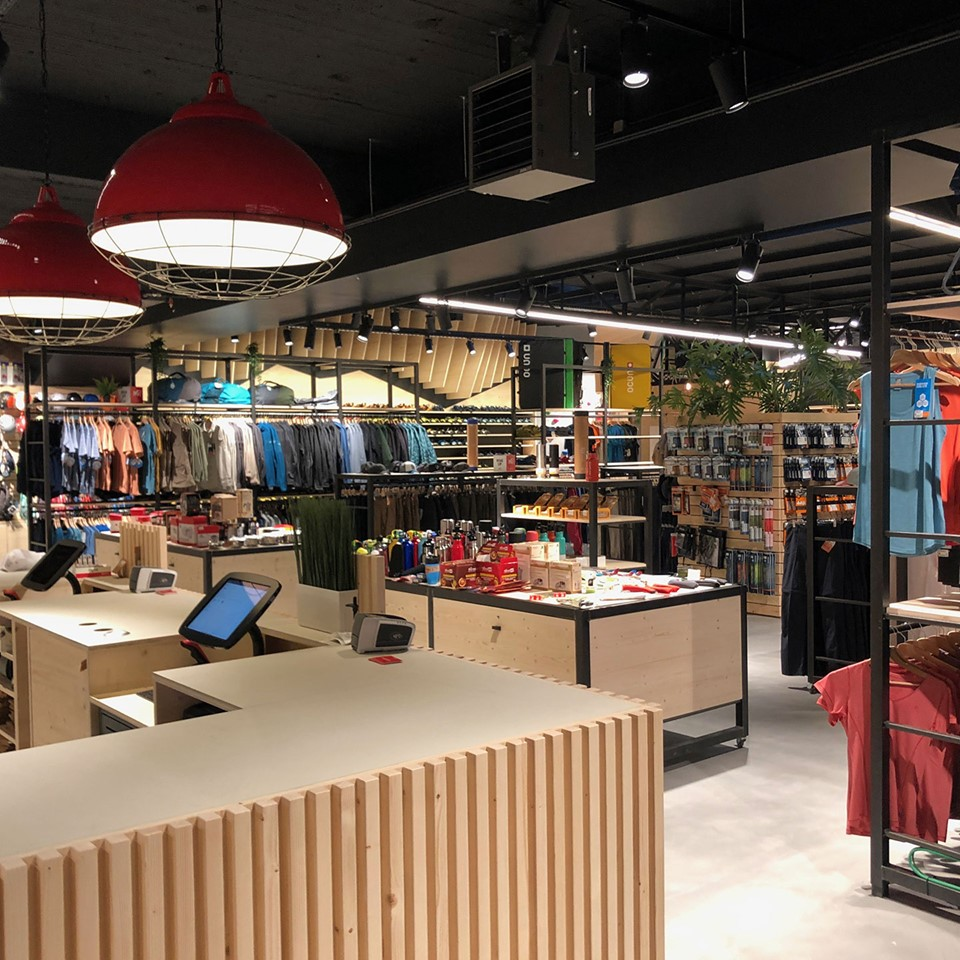
\includegraphics[width=\textwidth]{lecomte.jpg}
        \caption{Magasin Lecomte réalisé en mai 2019 à Ixelle, Bruxelles \href{https://www.facebook.com/Eclips.electricite/photos/a.1014356022289082/1014357662288918/?type=3&theater}{[5]}}
    \end{minipage}
\hfill
    \begin{minipage}[t]{.32\linewidth}
        \centering
        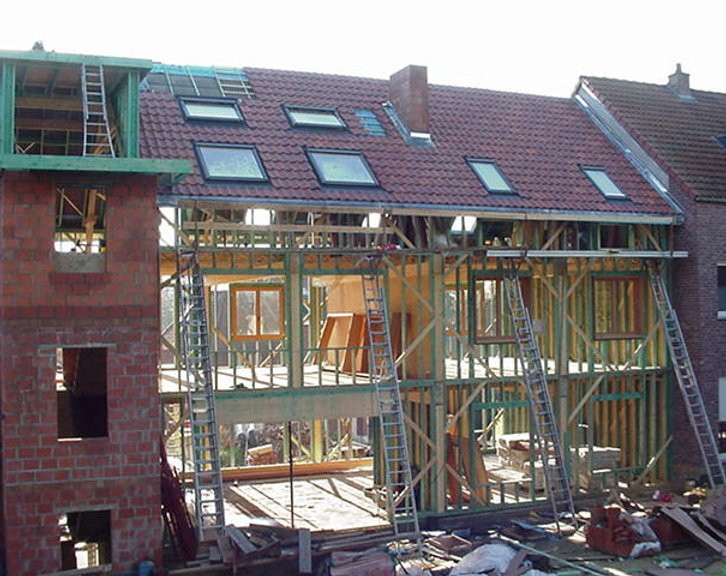
\includegraphics[width=\textwidth]{construction.jpg}
        \caption{Habitation ossature bois réalisée en 2013 à Boisfort, Bruxelles \href{https://www.eclips-sa.be/entreprise-gnrale}{[6]}}
    \end{minipage}
     \hfill   
     \begin{minipage}[t]{.32\linewidth}
        \centering
        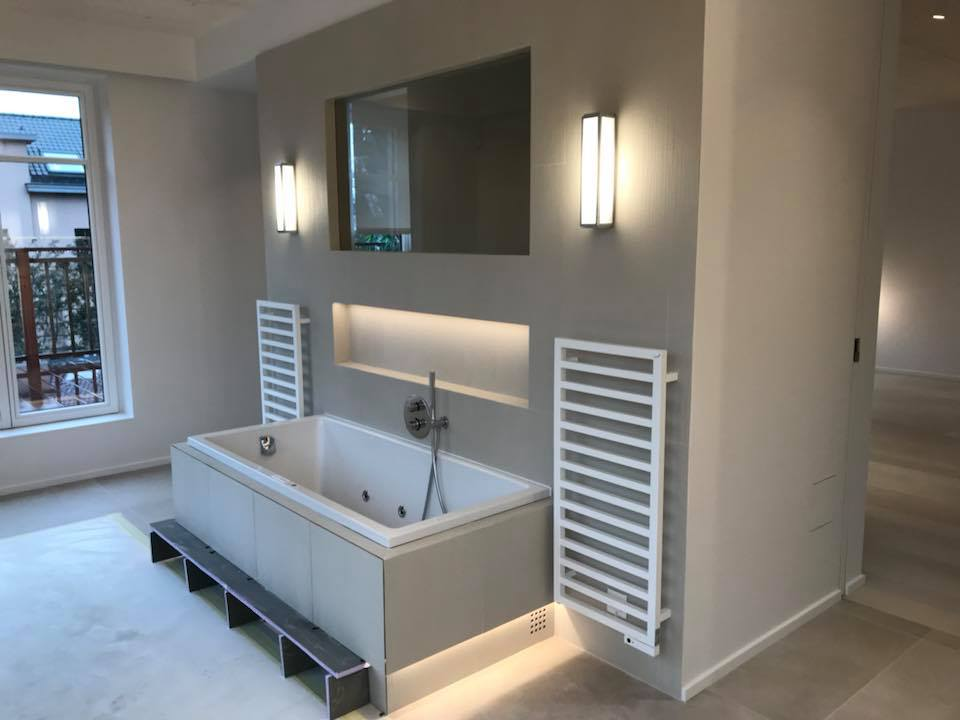
\includegraphics[width=\textwidth]{salle.jpg}
        \caption{Installation électrique réalisée en avril 2018 à Uccle, Bruxelles \href{https://www.facebook.com/Eclips.electricite/photos/a.675984922792862/679584145766273/?type=3&theater}{[7]}}
    \end{minipage}
\end{figure}

\subsection{Marché et communication}

La conjoncture du marché de la construction en date d'août 2019 sur la Belgique est représenté sur le graphique située en annexe \ref{appendix:b}. Selon la Banque Nationale de Belgique \href{https://www.nbb.be/doc/dq/f/dq3/histo/pfc1908.pdf}{[8]} : \\
\og{Le léger repli dans la construction, qui s’explique principalement par une contraction du carnet de commandes et par une moindre utilisation du matériel.\footnote{Par rapport à la courbe brute, la courbe lissée affiche un retard de quatre mois pour la branche d'activité construction.}}\fg\\

Sur ce marché, Eclips S.A. se porte relativement bien, le chiffre d'affaire est stable au fil des années. 
Elle opère sur une zone de chalandise s'étendant sur le sud de Bruxelles et sa périphérie élargie, une région plutot dynamique pour le secteur de la construction.\\

Les prestations sont effectuées en B-to-B pour les chantiers de grosse envergure et en B-to-C pour les interventions de plus petit calibre. Les deux types de clientèles ont décidé de coopérer avec Eclips principalement grâce une communication de type \og bouche-à-oreilles\fg, bien que l'entreprise communique via un site internet, une présence sur les réseaux sociaux et une inscription dans les bases de données de plusieurs constucteurs et fournisseurs.

\subsection{Concurrence et partenaires}

Le marché de la construction est un marché tendu au niveau de la concurrence, dû notamment à l'ouverture du marché aux acteurs européens \href{https://www.lesoir.be/art/803642/article/economie/immo/une-l-immo/2015-02-24/concurrence-deloyale-mine-secteur-construction}{[9]}\href{https://atradius.fr/publications/market-monitor-construction-belgique-2019.html}{[10]}, constituant une main-d'\oe{}uvre bien moins coûteuse que la main d'\oe{}uvre belge. Néanmoins, cette problématique impacte moins les professions qualifiées car elles sont protégées par des accès à la profession aux entreprises présentant les compétences du métier et de gestion requises. La principale solution pour avoir accès aux professions protégées est de présenter au moins un diplôme du métier et de gestion de base. \href{https://www.xerius.be/fr-be/devenir-independant/gestion-connaissances-professionnelles}{[10]}\\
Dans ce contexte-là et aussi par recherche de qualité, la concurrence ne se fait pas réellement sentir chez Eclips. Effectivement, dans le secteur de la construction de luxe, comme c'est souvent le cas en B-to-B, ce sont des lieux communs que la qualité se paie et qu'il est avantageux de fidéliser les prestataires compétents et éprouvés. J'ai déjà vécu des situations sur des chantiers pour des clients exigeants durant lesquels des sous-traitants, affichants des prix bien trop bas pour le marché, se faisaient renvoyer par l'entrepreneur général.\\

La société Eclips s'est construite avec un réseau d'entrepreneurs partenaires (électricien, plombier-chauffagiste, charpentier, entrepreneur général...), s'illustrant généralement avec la même culture de travail, à savoir professionnalisme et esprit familial. Bien souvent, les relations partenaires dépassent le cadre strictement professionnel, ce qui assure une meilleure coordination sur chantier et améliore encore un petit peu la qualité perçue. L'entraide se manifeste également lorsqu'un des entrepreneurs traverse une période un peu plus creuse, en sous-traitant l'une ou l'autre prestation pour assurer la continuité des affaires.

\section{Conclusion}

Eclips S.A. est sans doute une toute petite structure mais elle a su s'illustrer depuis une trentaine d'année sans rencontrer de difficulté majeure. Le professionalisme dont fait preuve la famille Canart dans ses réalisations est gage de pérennité dans les affaires et cela se vérifie dans les faits.\\L'âge de la retraite arrivant à grands pas pour François Canart, celui-ci se consacre maintenant plus activement à la sculpture métal - détails dans l'article en annexe \ref{appendix:c} - et s'efface peu à peu du secteur de la construction générale. Paradoxalement, cette nouvelle activité, exercée au nom d'Eclips, est florissante et assure des rentrées d'argent appréciables.\\La continuité de l'entreprise en électricité est également assurée par une comptabilité rigoureuse et par un carnet de commandes rempli, issues de clients présentant divers profils. Cette diversification permet d'encaisser les aléas du marché plus sereinement que des entreprises en électricité spécialisées dans tel où tel domaine et parfois plus fragilesface à des récessions ou de décisions politiques hasardeuses. \href{https://www.rtl.be/info/regions/brabant-wallon/les-entreprises-de-photovoltaique-continuent-de-tomber-sunswitch-fait-faillite-60-emplois-perdus-414257.aspx}{[11]}\\

De part l'incursion priviliégée dans le secteur de la construction que le Compagnonnage m'octroie, je peux sans forcer le trait témoigner d'une culture d'entreprise plutôt exceptionnelle pour le secteur, et également qu'il ne faut pas nécessairement officier dans une énorme structure pour bénéficier des meilleures conditions de travail.\\

\newpage

\part{Activité : chef d'entreprise installateur électricien}

\setcounter{section}{0} 

 \section{Introduction}

C'est un choix bien à contre-courant que de présenter des activités d'électricien en bâtiment plutôt que d'électrotechnicien en industrie. Et pourtant, dans cette entreprise, bien que la technicité ne fut pas d'un niveau élevé, j'ai eu l'occasion de gérer des chantiers en totale autonomie, du devis à la réception du chantier, de découvrir les tenants et aboutissants de la domotique ou encore de gérer une petite équipe de deux ouvriers. A mon sens, toutes ces tâches remplissent bien mieux les fonctions que peut assumer un technicien supérieur en électrotechnique, par rapport aux missions que j'ai pu effectuer dans d'autres entreprises.\\

Chez Eclips, j'ai officé de 2016 à 2019. J'ai débuté comme apprenti installateur électricien, assorti dans une formation qualifiante belge intitulée \og Chef d'Entreprise Installateur Electricien \fg{} au centre de formation bruxellois EFP.  Cette formation en alternance dure trois ans et doit permettre à ceux qui en sortent de monter une entreprise en électricité. Elle octroie donc des compétences métier niveau Bac Pro ELEEC et des compétence en gestion de base d'une entreprise. Il s'agit typiquement de formation donnant l'accès à la profession.\\

A la fin de la première année, j'ai terminé mon apprentissage en validant l'examen C (équivalent du CAP en Belgique) et j'ai souhaité continuer de travailler chez lui jusqu'à la fin de ma formation. En parallèle de cela, j'ai également validé en candidat libre un Bac Pro ELEEC mention Très Bien en juin 2018. Et j'ai ensuite entamé une première année de BTS électrotechnique en candidat libre également pour valider les matières générales du diplôme avant de partir sur le tour de France.\\

 
 \section{Situations et tâches}

Suivant le programme de ma formation Chef d'Entreprise Installateur Electricien, mon patron Maxime Canart a très bien respecté sa mission de me donner toutes les clés en main pour monter et pérenniser une entreprise en électricité dans sa globalité. En ce sens, les tâches effectuées sont les mêmes que celles que mon patron effectue pour assurer le bon fonctionnement de son entreprise d'installation en électricité, à savoir :

\begin{itemize}

  \item Etude de projet et dimensionnement en fonction du cahier de charge ;
  \item Conseil client en électricité générale et éclairagisme ;  
  \item Mise et remise en conformité au regard des normes en vigueur ;
  \item Chiffrage et élaboration de devis ;
  \item Gros-\oe{}uvre (saignée, carottage, préparation au câblage...) ;
  \item Câblage (courant fort, parlophonie, GTB, VDI, alarme, domotique, multimédia...) ;
  \item Eclairage (suspension, encastré, bandeau LEDs, éclairage extérieur...) ;
  \item Armoire électrique (montage, câblage, programmation, baie de brassage...) ;
  \item Plan (repérage, schéma des installations électrique...) ;
  \item Mise en service (mesures de test au regard des normes en vigueur) ;
  \item Service après-vente (dépannage et amélioration d’installation existante) ;
  \item Gestion d'équipe (organisation de chantier avec le client, les sous-traitant et les fournisseurs..) ;
  \item Gestion d'entreprise (gestion des stocks, commande...).
    
\end{itemize}
Ces tâches sont effectuées en horaires de travail classique, 40 heures par semaines (horaire usuel en Belgique) et les cours de la formation Chef d'Entreprise Installateur Electricien furent dispensés en cours du soir.

\subsection{Tâche n\degree1 : domotique}

\subsubsection{Présentation générale}

Eclips S.A. propose à ses clients une installation électrique de type domotique, amenant à un plus grand confort d'utilisation et une évolutivité pour les installations électriques du bâtiment.\\
Début 2017, tout le personnel de la branche électricité d'Eclips a suivi les modules de formations octroyés par le fabriquant Niko pour agréer l'installation de leur solution domotique propriétaire Niko Home Control (NHC).\\ Cette solution s'apparente à une solution de type KNX \href{http://www.knx.fr/KNX-France-quest-ce-que-knx.html}{[12]} mais propose une approche de la programmation beaucoup plus simplifiée, dont la maîtrise s'acquiert en trois sessions de formation pour les installateurs électriciens.

 \begin{figure}[h]

\includegraphics[scale=0.1]{NHC1.jpg}
\centering
\end{figure}

\subsubsection{Qualités/défauts \& conception}

Les installations électriques domotiques sont particulièrement intéressantes pour la gestion énergétique des grosses habitations. Elles présentent divers qualités et défauts par rapport aux installations électrique domestiques en logique cablée :

\setlength{\doublerulesep}{0pt}
\begin{tabularx}{\textwidth}{X X}
\hline\hline

\textbf{Qualités} & \textbf{Défauts}\\

\endhead
\hline

Evolutivité et connectivité&Coût du matériel et alourdissement de l'installation\\
Confort d'utilisation &Complexité d'utilisation (si mauvaise installation)\\
Sécurisation de l'habitation&Image parfois \og gadget \fg et usine à gaz\\
Gestion et économie d'énergie&Crainte d'une attaque informatique\\
Facilité de programmation pour les solutions propriétaires&Complexité de programmation pour les solutions de type KNX\\
Centralisateur des techniques du bâtiment (multimédia, moteur, VMC, alarme, contrôle d'accès...)&Maintien du système à jour par le constructeur pour les solutions propriétaires      \\
Ouverture et évolution du protocole de communication à plusieurs fabriquants pour les solutions KNX& \\
\hline\hline
\end{tabularx}

Un système domotique complet s'articule de manière générale autour d'une unité centrale à laquelle sont connectés différents modules de commande et communication et un bus connecté à divers unités de commandes adressables et/ou programmables. Un tel système est similaire à une installation industrielle automatisée.\\Un solution ouverte de type KNX présente l'avantage de réunir plusieurs fabriquants autour d'un même protocole de communication, tandis que les solutions propriétaires comme NHC présentent l'avantage d'être beaucoup aisément programmables mais plus restreintes en termes de fonctionnalités.\\

Chez Eclips, comme nous avons un certificat d'installateur NHC, on présente au client en premier lieu 
cette  solution, même si l'entreprise est tout à fait qualifiée pour installer n'importe quel solution, sur conseil du fabriquant. La programmation de l'installation sous KNX est quant à elle réalisée par un sous-traitant le cas échéant.\\Installant principalement cette solution, je détaillerai ici les principes de conception, de réalisation et de programmation de Niko, bien que le principe soit relativement identiques pour les autres solutions diffusées sur le marché.\\

Niko Home Control est la solution domotique du fabriquant de matériel électrique belge Niko, leader sur le marché belge du matériel électrique pour le particulier, commercialisant du matériel électrique de qualité. La firme propose un système d'installation électrique connecté NHC qui est une solution propriétaire qui permet de connecter son installation électrique pour améliorer le confort (utilisation, scène d'éclairage, connectivité...), l'efficacité (monitoring, gestion du chauffage...) et la sécurité (contrôle d'accès, alarme...) de l'habitation. Elle établit régulièrement des passerelles de communication avec différents constructeurs pour rendre son installation intégrée de manière optimale vis-à-vis des autres techniques du bâtiment (Velux, Sonos, IFTTT, Bose, Bulex, Vaillant...).\\Pour les plus programmateurs, Niko a diffusé une API (\textit{Application Programming Interface}) permettant à l'installation connectée de communiquer avec des unités de contrôle type Raspberry Pi ou l'interface Apple HomeKit via le protocole de communication MQTT. \href{https://www.niko.eu/fr-be/nos-produits/automatisation-domestique}{[13]}

\subsubsection{Réalisation}

Pour réaliser une installation domotique, il faut tout d'abord identifier les besoins du client, ce qui permet de dimensionner et orienter les fonctions que présenteront l'installation (sécurité, confort et économie).

\paragraph{Câblage}
~\\
Ce type d’installation présente la particularité de ramener à l’armoire électrique chaque alimentation de point lumineux, prise ou tout autre appareil à commander, ce qui alourdit l'installation par rapport à une installation en logique câblée classique.\\

Les photos ci-contre explicitent les différentes étapes de la réalisation d’un tableau domotique sur un villa situé dans la banlieue de Bruxelles, qui commande qu’un seul étage de cette habitation.\\
Le câblage est ramené au tableau et comprend :

\begin{itemize} 
  \item Circuits de courant fort non commandés et le câblage classique d'une installation traditionnelle ;
  \item Chaque circuit de courant fort à commander (éclairage et prise) ;
  \item Le bus entre les bouton-poussoirs adressables, avec une topologie en boucle ou en étoile ;
  \item Les différents câbles de commandes (VMC, chauffage, VDI, liaisons entre les tableaux...) et de puissances (stores, volets...).
\end{itemize}

Chaque câble doit être correctement identifié et il faut faire preuve d’organisation dans l’agencement des bottes de câbles pour optimiser l’espace dans le tableau. Les normes électriques restent en vigueur pour les circuits en 230V, tandis que les circuits de commandes alimenté en 26V par le bus ne sont pas soumis aux mêmes réglementations.\\Le bus est câblé en boucle ouverte pour permettre de dépanner facilement l’installation en cas de sectionnement du bus, puisqu’il suffit de brancher le retour de la boucle du bus pour reconnecter le bus aux platines de contrôles.\\

\begin{figure}[h]
    \begin{minipage}[t]{.46\linewidth}
        \centering
        \includegraphics[width=\linewidth]{cablage1.jpg}
        \caption{répartition des circuits électriques dans l'habitation}
    \end{minipage}
    \hfill
    \begin{minipage}[t]{.46\linewidth}
        \centering
        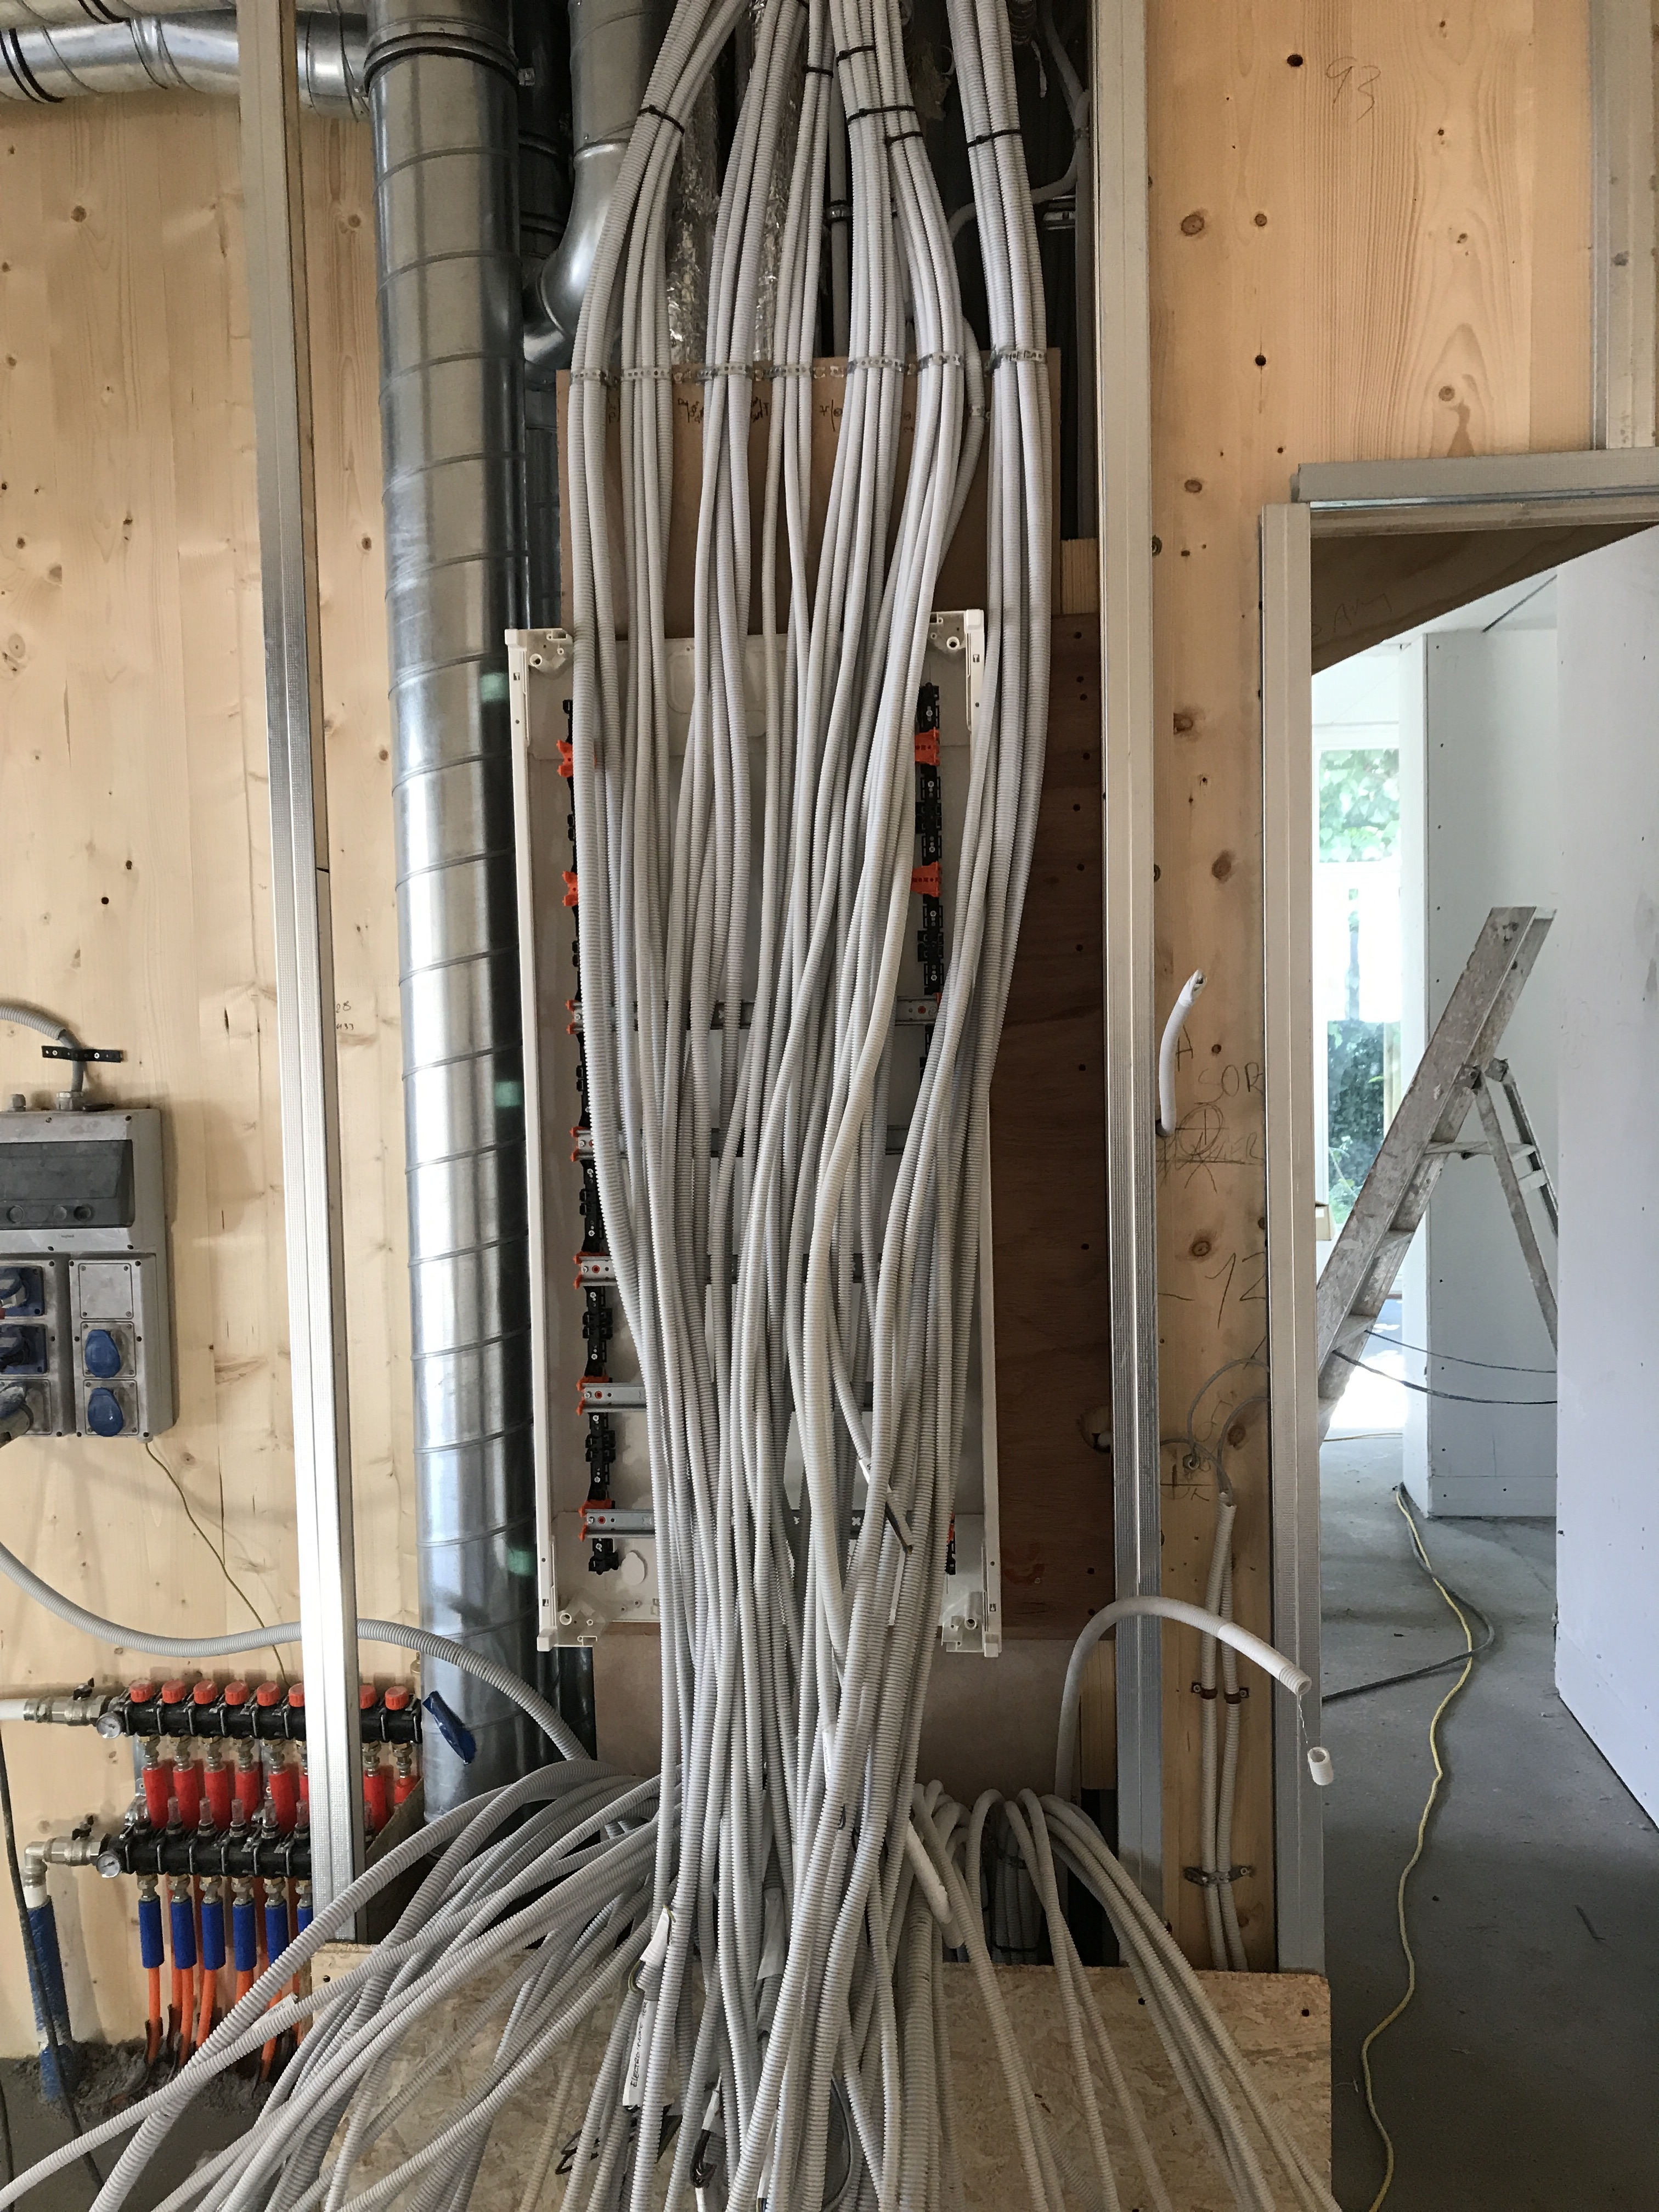
\includegraphics[width=\linewidth]{cablage2.jpg}
        \caption{Organisation des circuits électriques dans le tableau}
    \end{minipage}
\end{figure}

\paragraph{Tableau}
~\\
L’armoire électrique est montée en deux parties distinctes :
\begin{itemize} 
  \item Puissance
  \begin{description} 
  \item[Non commandée :] les circuits de puissance non commandés sont disposés conformément aux normes en vigueur et sont indépendants de l’installation domotique ;
  \item[Commandée :] les circuits de puissance commandés sont répartis sur un bornier et numérotés en prenant bien soin de vérifier la bonne attribution des câbles. Les modules de commutation NHC étant constitués de contacts unipolaires, le neutre de chaque circuit protégé par un disjoncteur peut être disposé sur un bornier de neutre.
\end{description} 

\item Commande\\
Les modules de commandes sont regroupés ensemble et connectés afin qu’ils puissent communiquer. Un disjoncteur alimente les contacts de puissance d’un, voire deux module(s) de commande selon le nombre de points.\\Ce tableau présente un panel de fonctions fréquemment rencontrées en domotique :
\begin{description} 
  \item[Commutation :] six éclairages différents par module ;
  \item[Gradateur :]  deux éclairages différents par module ;
  \item[Moteur :] trois moteurs de volet ou store par module ;
  \item[VMC :] commande de la VMC ;
  \item[Chauffage :] commande d'électrovannes ;
  \item[Alarme :] liaison permettant à l’installation de réagir à une intrusion détectée par l’alarme (simulation de présence, diffusion d'alarme via l'installation multimédia...).
\end{description} 
\end{itemize}

Une unité de contrôle connectée à Internet se charge de gérer l’installation dans son
ensemble en local et à distance.

\begin{figure}[h]
    \begin{minipage}[c]{.46\linewidth}
        \centering
        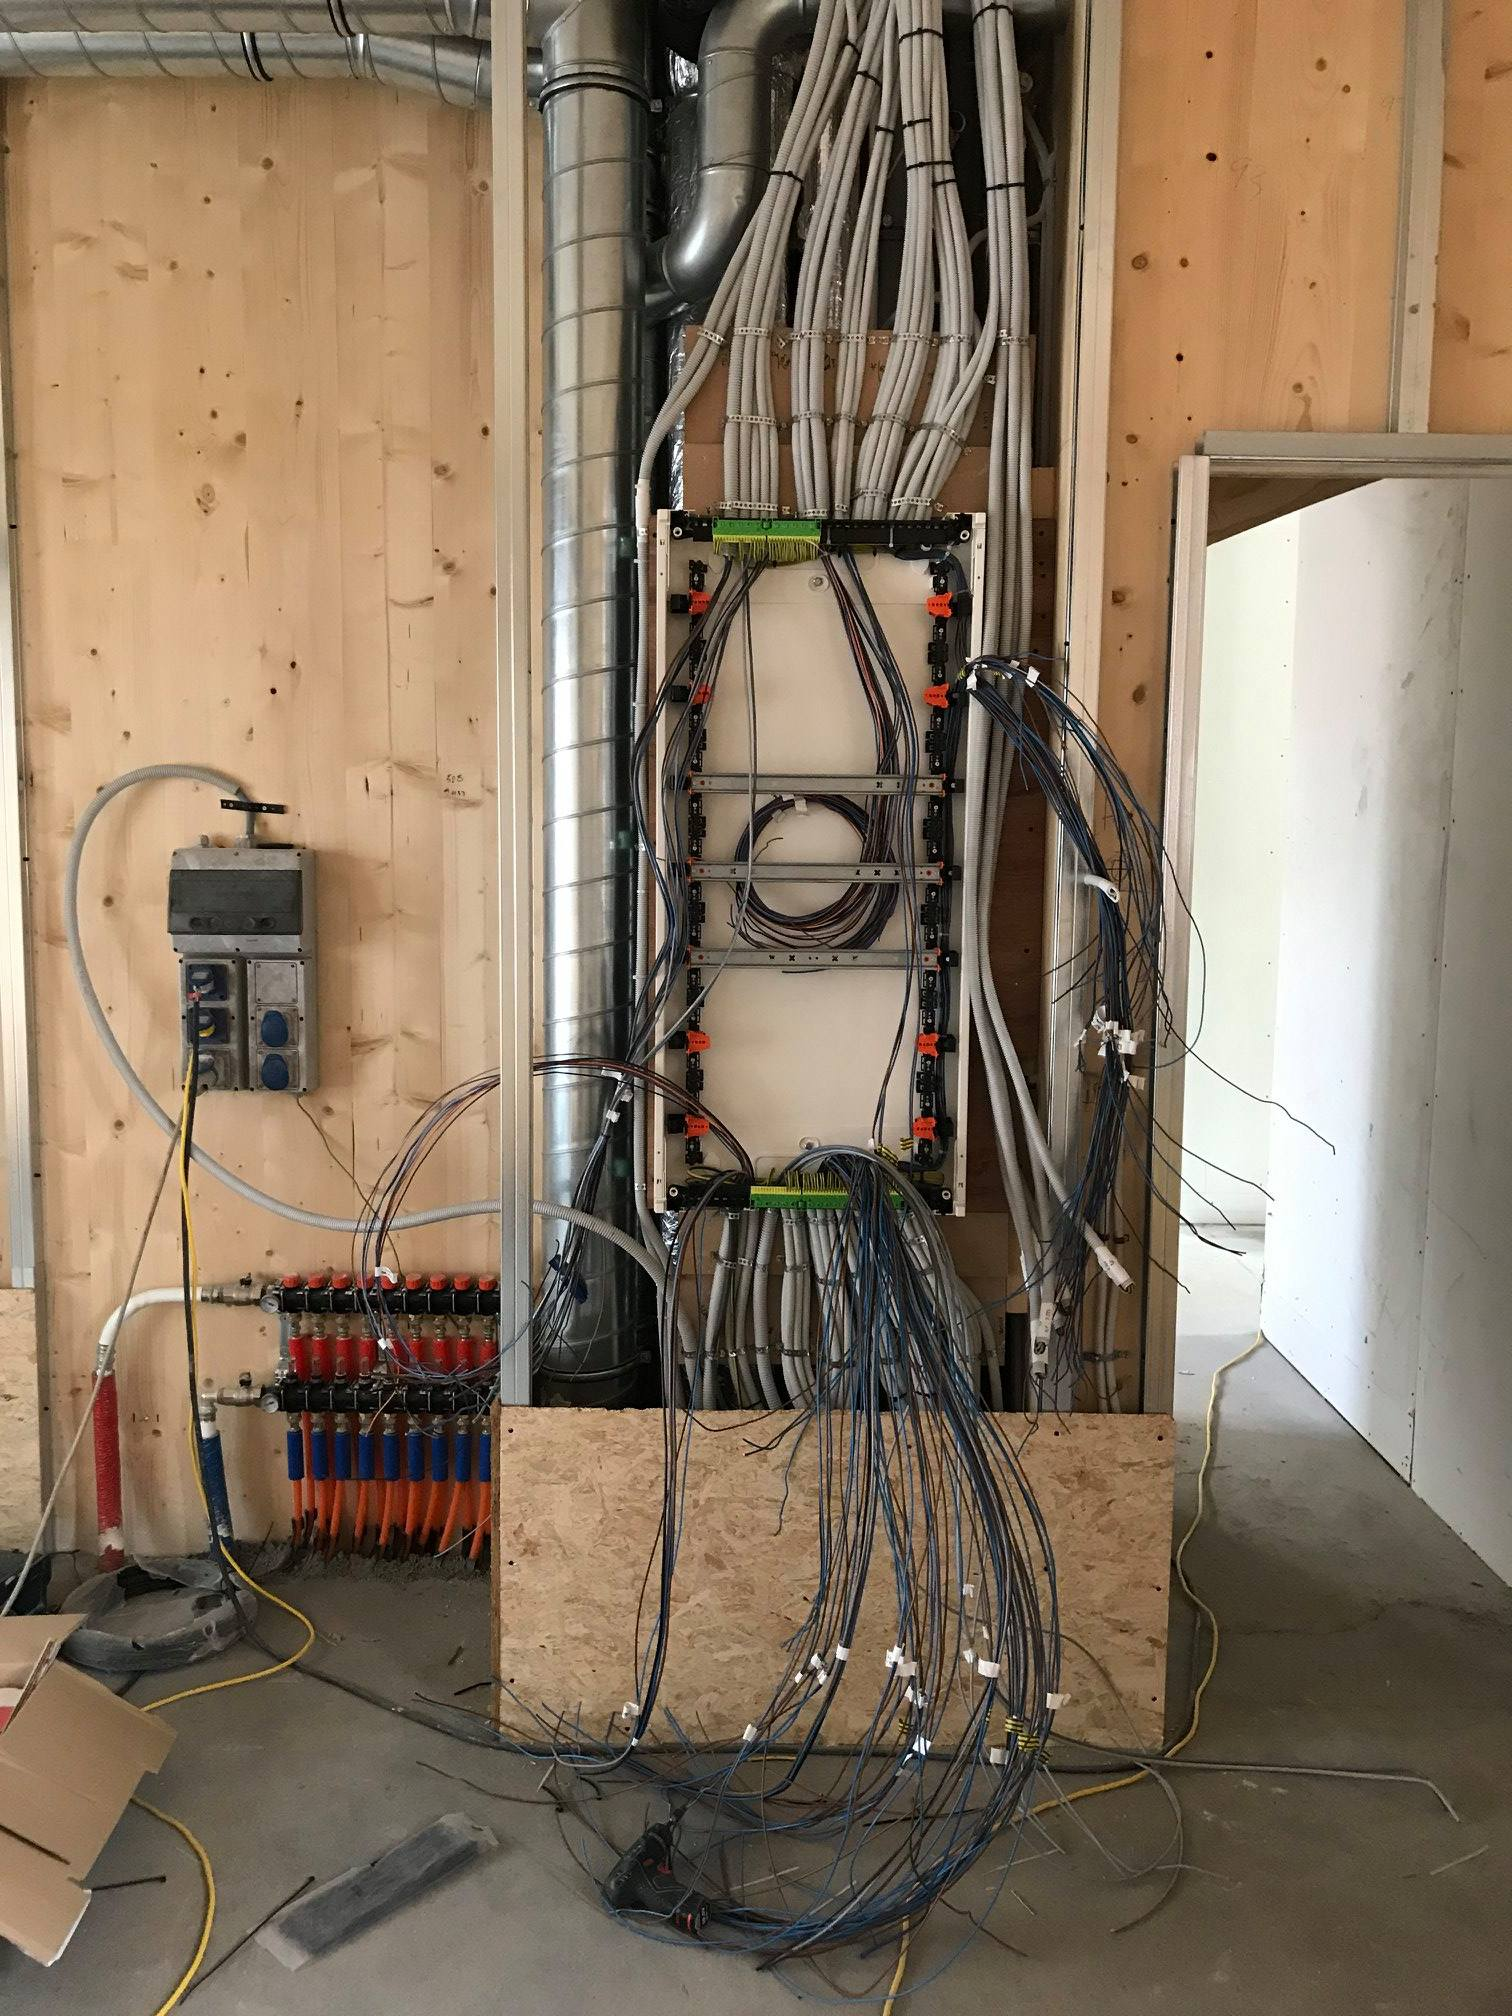
\includegraphics[width=\linewidth]{armoire1.jpg}
        \caption{Prépration du cablâge}
    \end{minipage}
~
    \begin{minipage}[c]{.46\linewidth}
        \centering
        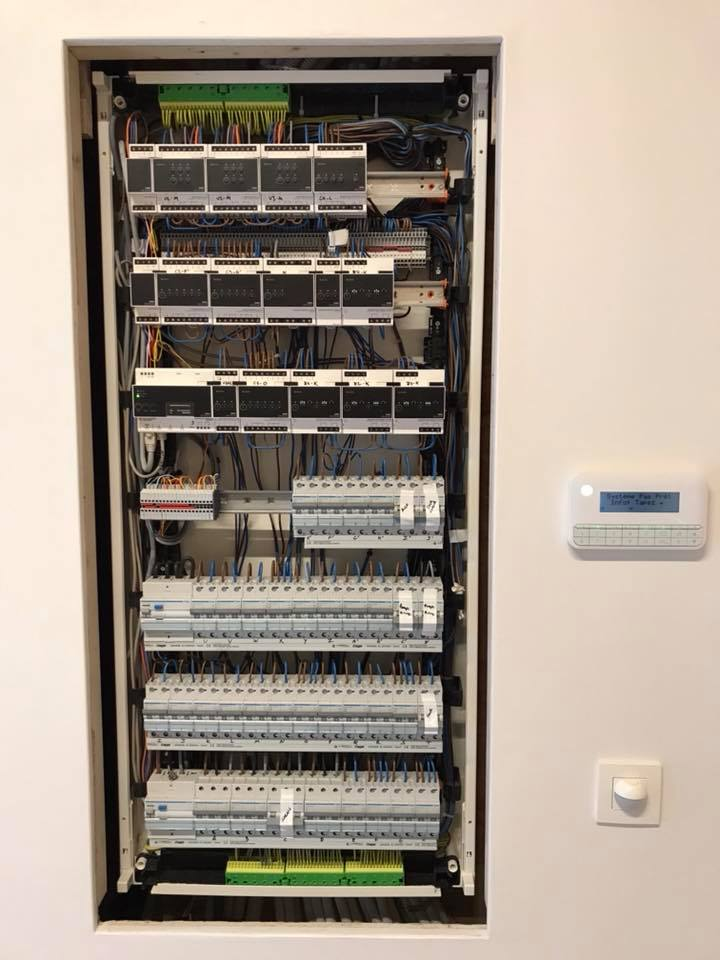
\includegraphics[width=\linewidth]{armoire2.jpg}
        \caption{Finalisation du tableau}
    \end{minipage}
\end{figure}

\subsubsection{Programmation}

L’installation domotique est programmée à l’aide d’un logiciel qui est beaucoup plus simple et intuitif que le KNX standard, avec le défaut qu’il soit propriétaire et qu’il présente moins de possibilités de personnalisation.\\Le principe de ce type d’installation est que chaque bouton-poussoir, application sur smartphone, écran tactile... peut potentiellement contrôler tous les points commandés de l’installation.\\

Le client peut décider, épaulé par la société, de configurer ses éclairages et autres appareils à son envie. Fort des formations suivies chez Niko, nous pouvons conseiller différentes programmations telles que des simulations de présences, des horaires de chauffages, des tout-off, des temporisations des VMC par zone...\\La pertinence de la programmation et ses fonctions spécifiques fera la différence chez le client, pour peu qu’il porte de l’intérêt à ce type de fonctionnalité. En annexe \ref{appendix:d} se situe un exemple de l'interface de programmation du logiciel NHC II.

\subsubsection{Conclusion}

Cette situation de travail fut moins fréquente, mais autrement plus motivante tant le fait de travailler sur des éléments évolutifs et programmables me passionne.
Ces réalisations-là diffèrent assez bien des mises en conformité et peuvent paraître moins indispensable en habitat. Et pourtant, dans le domaine tertiaire, les techniciens sont beaucoup plus souvent confrontés à ce type d’installation et en industriel, le principe de fonctionnement des automates programmables industriels est similaire à celui des installations domotiques.
Cela, mon patron l’avait bien saisi et m'a laissé beaucoup d’autonomie dans ces réalisations pour me permettre d’apprendre un maximum.

\subsection{Tâche n\degree2 : entrepreunariat en électricité}

\subsubsection{Introduction}

Etant en fin de formation Chef d'Entreprise Electricité, il me fallait apprendre également à gérer des affaires de A à Z en électricité. Cela a été rendu possible par la confiance que m'a accordé mon patron. J'ai donc eu l'occasion de réaliser une installation électrique en nom propre, la société fournissant seulement une facture pour rester dans la légalité et assurer l'installation.

\subsubsection{Chiffrage}

Un client a fait appel à mes services pour réaliser une installation électrique neuve dans une petite maison d'habitation en location, l'ancienne installation étant complètement vétuste. Comme ça peut souvent être le cas pour les petites affaires, nous avons conclu que le chantier se reglèrait au prix catalogue pour le matériel et en régie pour une intervention estimée à une durée de 50 heures, au taux horaire de 40\EUR/heure.

\subsubsection{Commande et outillage}

Pour la commande, en référence au devis établi, j'ai réalisé une commande de matériel chez le fournisseur Rexel. Concernant l'outillage, étant déjà correctement équipé, je n'ai que quelques outils spécifiques à emprunter à Eclips, dont un testeur de terre.

\subsubsection{Réalisation}

La réalisation s'est déroulée sans accroc particulier mais dans des conditions difficiles car l'habitant restait sur place et l'espace était relativement restreint. J'avais estimé une durée de 50 heures pour la réalisation et ce fut une estimation pile poil correcte, l'intervention a duré une semaine.\\
J'ai fait appel à mon collègue pour une journée de travail, pour éviter de déborder sur le week-end et j'ai donc du l'encadrer pour qu'il réalise les tâches assignées correctement.\\

Le client souhaitant une installation nécessitant le moins de gros-\oe{}uvre possible, j'ai suggéré de réaliser l'installation en saillie mais sous gaine, et qu'une fois la locataire partie, il serait possible de cloisonner les murs et encastrer les gaines. La suggestion fut acceptée et cela m'a permis d'éviter une charge de gros-\oe{}uvre trop importante.\\

\begin{figure}[h!]
	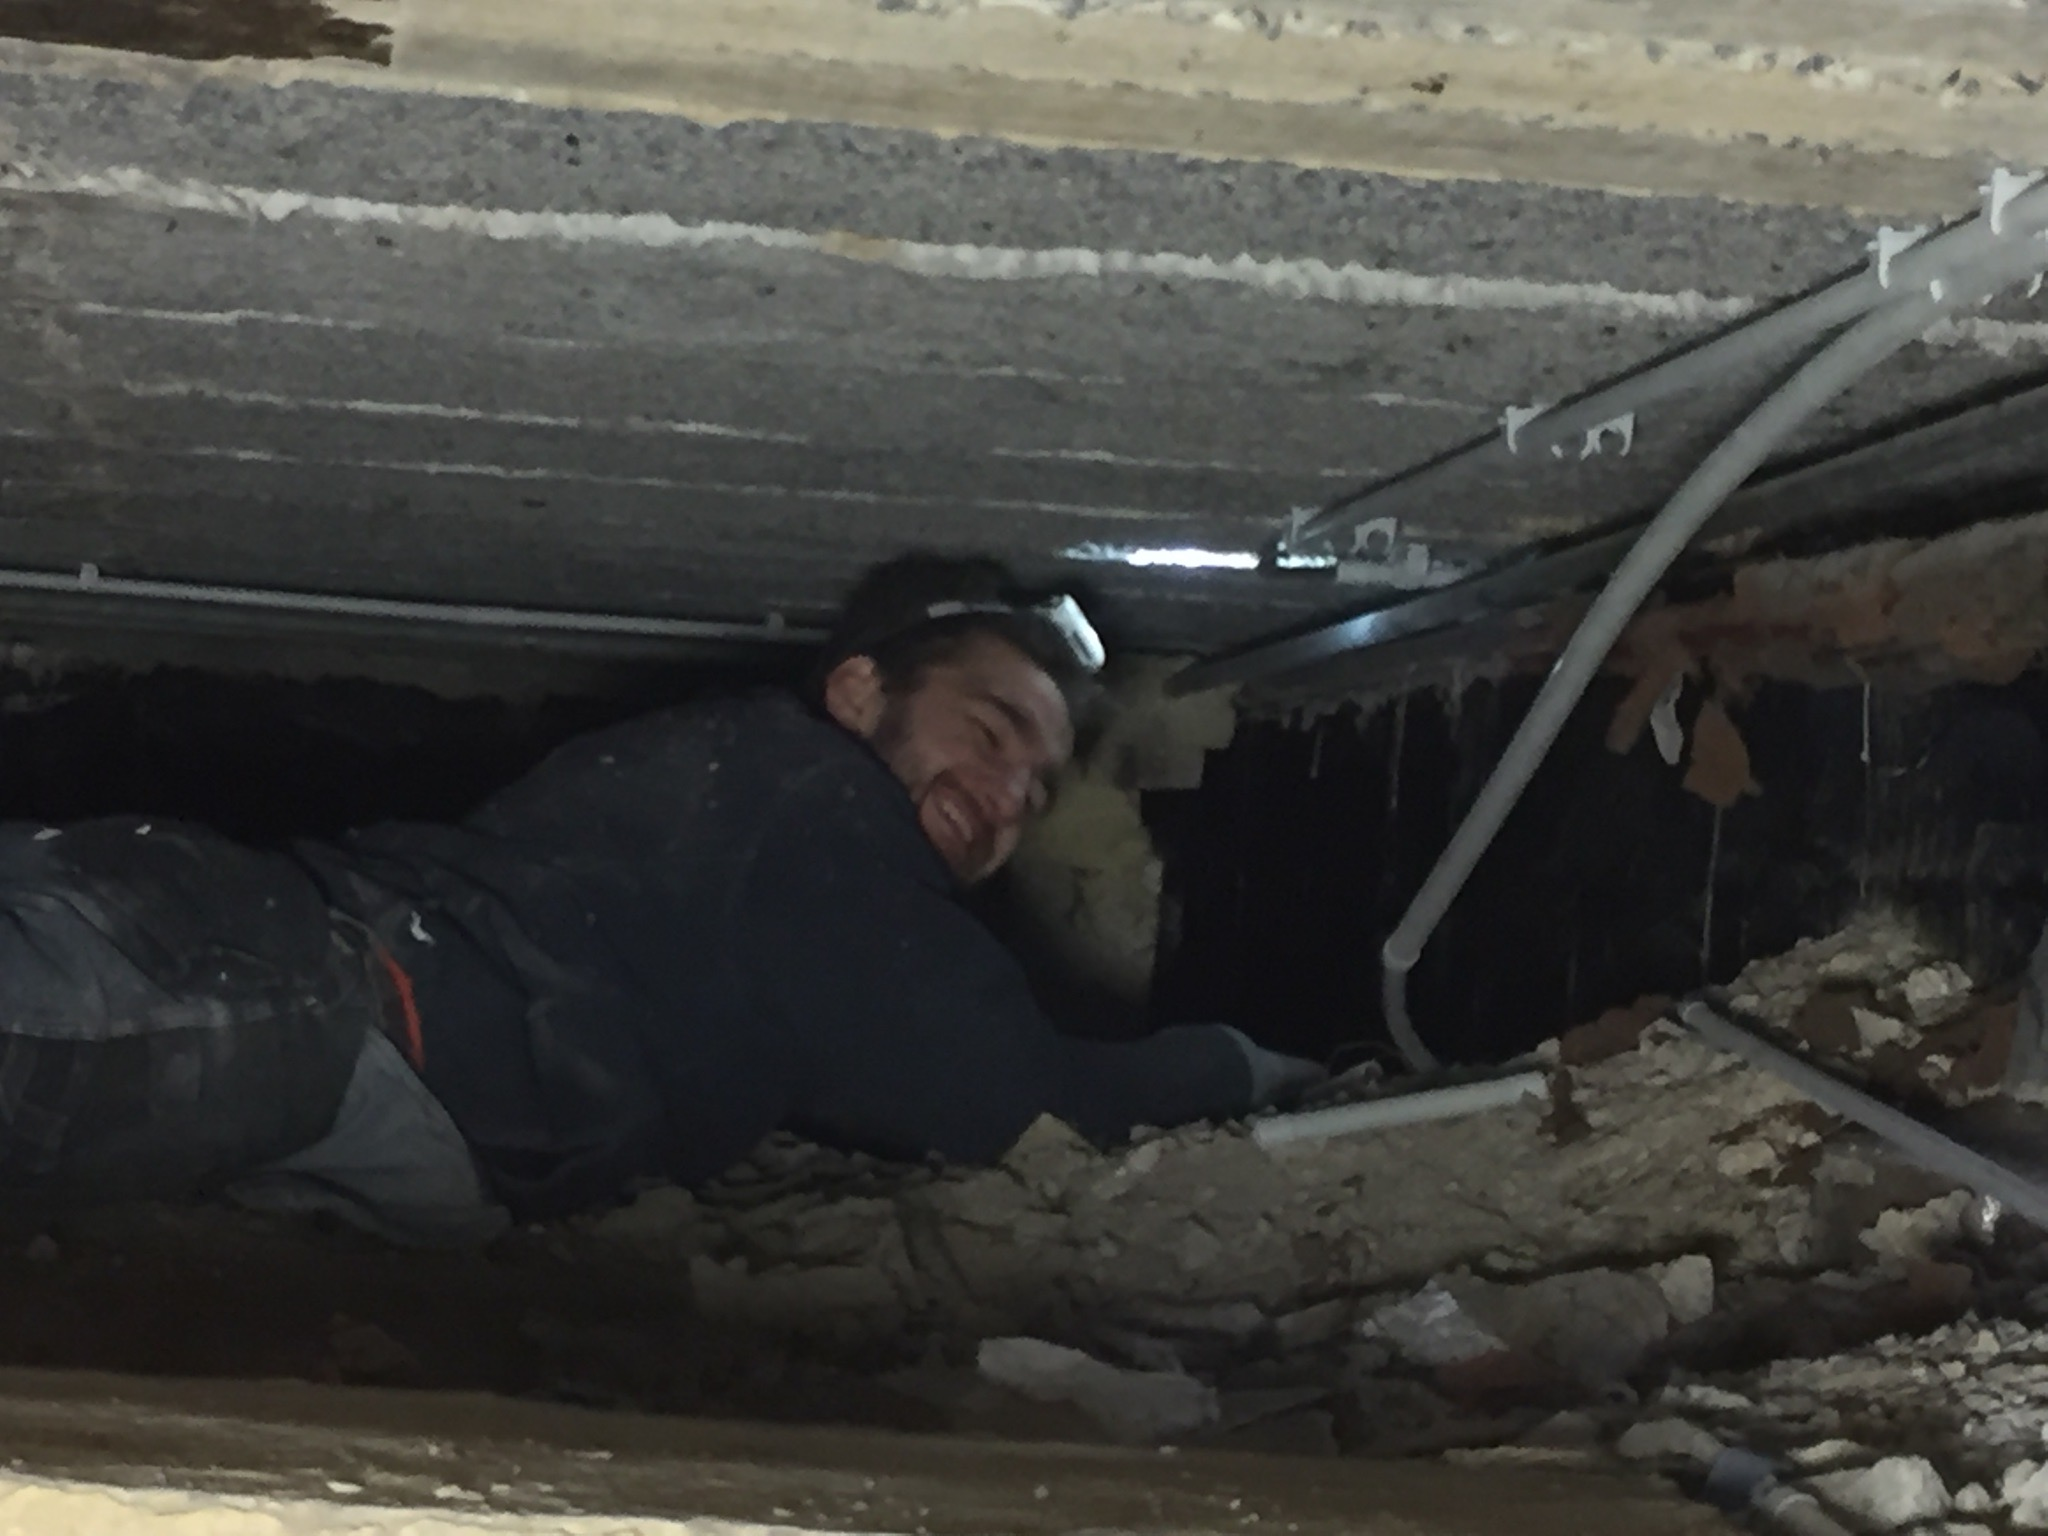
\includegraphics[scale=0.12]{videtechnique.jpg}
		\centering
		\caption{Passage de câbles en vide ventilé}
\end{figure}

\subsubsection{Conformité}

Selon le devis et dans ma déontologie de travail, l'installation électrique devait évidemment être réceptionnée conformément aux normes en vigueur, le Règlement Général sur les Installations Electriques (RGIE) \href{https://www.legrand.be/montage/fr/rgie}{[14]}, l'équivalent belge de la norme NF C15-100. \href{https://www.legrand.fr/pro/normes-et-reglementations/norme-nf-c-15-100/norme-nf-c-15-100-suivez-le-guide}{[15]}\\

Les normes en vigueurs en Belgique sont relativement similaires sur le fond, avec une différence notoire sur la valeur de la terre, qui doit être inférieure à 30 Ohms en Belgique et 100 Ohms en France. La répartition du tableau est donc simplifiée à deux interrupteurs différentiels, un en tête d'installation d'une sensibilité de 300mA et l'autre pour les zones humides d'une sensibilité de 30mA.\\Il existe une autre différence entre la France et la Belgique au niveau du mode de distribution du courant. En Belgique, le réseau électrique étant majoritairement distribué en biphasé (tension composée $U=230V$), les disjoncteurs magnétothermiques doivent donc présenter une protection bipolaire, phase et (faux) neutre.\\Par commodité, un faux neutre repéré en bleu est systématiquement utilisé. Les disjoncteurs sont généralement deux fois plus épais qu’en France et cela tend à rendre les tableaux de distribution plus volumineux en Belgique.\\En France, le réseau est distribué en minimum monophasé 400V + neutre. Seule la phase est protégée par un disjoncteur, le vrai neutre y attenant étant protégé par un contact commandé par la protection de la phase.\\Une dernière différence concerne la réalisation de plans. Un dossier contenant un plan unifilaire, de position et la description des circuits électriques dans l'habitation est obligatoire pour l'obtention du certificat de conformité en Belgique. Il est délivré au contrôleur, au client et conservé par l'installateur. Ce dossier permet un repérage aisé d'un éventuel circuit en défaut.\\

Pour le reste, les réglementations se valent à quelques nuances près :

\begin{description}

\item[Dimensionnement :] section de câble de 1,5mm\up2 minimum pour les circuits d’éclairages, 2,5mm\up2 minimum pour les circuits de prises et mixte, 4mm\up2 minimum pour les circuits d’alimentation triphasée des taques électriques, 6mm\up2 pour les circuits d’alimentation monophasée des taques électriques... ;
\item[Câblage :] respect des modes de poses correspondant au type de câble électrique, respect des volumes humides... ;
\item[Distribution :] 8 points de prises maximum par circuit, calibre et courbe du disjoncteur adaptés au circuit à protéger, présence de circuits spécialisés pour les appareils ménagers, disjoncteurs et interrupteurs différentiels répondant aux normes en vigueur, tableau électrique fermé par une porte et obturé par des caches, indications de sécurité réglementaires, identification des circuits électriques... ;
\item[Protection :] protection de l’installation via un différentiel 300mA en tête d’installation, protection des personnes via un différentiel 30mA pour les locaux humides et machine en contact avec de l’eau... ;
\item[Mise à la terre :] sections et couleurs adéquates des câbles et de la mise à la terre, liaisons équipotentielles pour les carcasses métalliques, résistance de terre inférieure à 30 Ohms, présence d’un piquet de terre... ;
\item[Isolation :] la mesure d’isolement générale de l’installation entre
les phases et la terre doit être supérieure à $R_{test}=1000V_{test}$;
\item[Plan de l’installation :] schéma unifilaire et de position de l’installation électrique (en annexe \ref{appendix:e}).

\end{description}
\begin{figure}[h!]
    \begin{minipage}[t]{.43\linewidth}
        \centering
        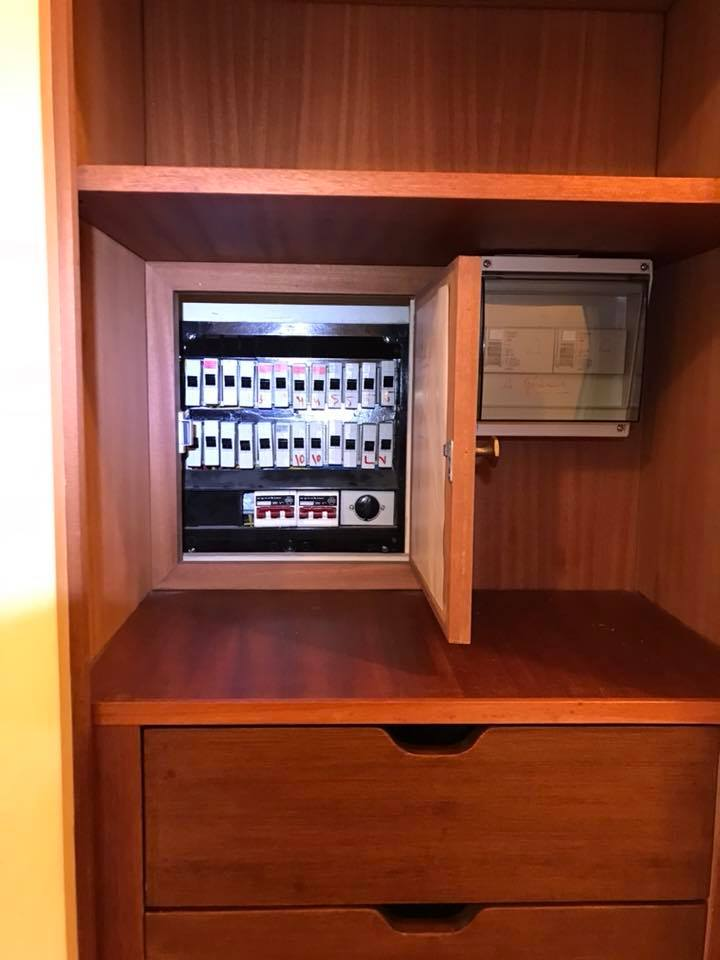
\includegraphics[width=\linewidth]{conformite1.jpg}
        \caption{Tableau électrique avant intervention}
    \end{minipage}
    \hfill
    \begin{minipage}[t]{.43\linewidth}
        \centering
        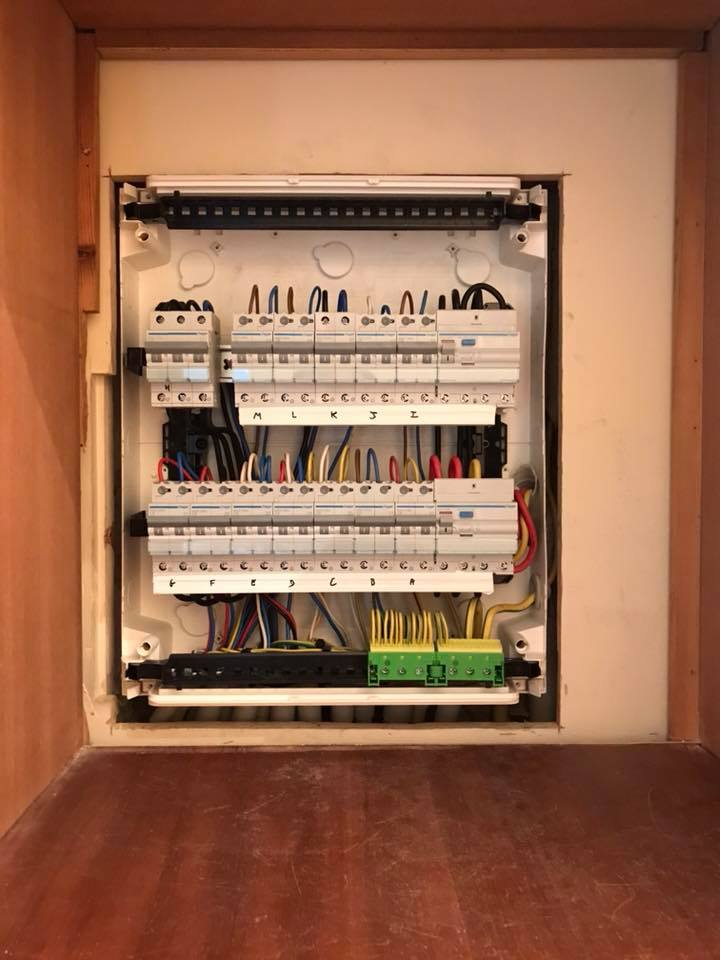
\includegraphics[width=\linewidth]{conformite2.jpg}
        \caption{Tableau électrique après intervention}
    \end{minipage}
\end{figure}

Pour l'affaire détaillée ici, l'installation était tellement vétuste que mon intervention en est devenue primordiale pour la sécurité du locataire face aux risques d'incendie d'origine électrique.\\Pour exemple, voici le tableau électrique que j'ai remplacé lors de l'intervention, il est complètement vétuste et ne réponds plus du tout à la dernière version du RGIE :
\begin{itemize}
\item Disjoncteurs monophasés type « Mini-Jump » à broches, de calibres différents sur les phases et le neutre des mêmes circuits ;
\item Protections ne répondant plus aux dernières versions du RGIE ;
\item Porte bricolée en bois (propagateur de la flamme), ouvertures non obturées dans le tableau.
\end{itemize}

\subsubsection{Conclusion}

Cette expérience s'étant déroulée sans accroc, s'ensuivit alors des réalisations similaires tout le long de l'année 2019-2020, qui furent toutes aussi concluantes.\\ Cette situation de travail résume ainsi trois années passée chez Eclips et crédibilise également le bien-fondé de la formation Chef d'Entreprise, validé scolairement par un travail de fin d'étude effectué en fin d'année 2019, qui consistait en un montage d'une entreprise fictive et la réalisation d'une grosse affaire en électricité secteur habitation domestique.\\Les circonstances ne se ressemblant jamais, j'ai donc appris chez Eclips à faire preuve d'initiative et d'imagination pour trouver une solution aux (nombreuses) problèmatiques rencontrées sur chantier et pour trouver une solution satisfaisante aux attentes parfois farfelues des clients. La sacro-sainte règle d’application chez Eclips reste toutefois de toujours parvenir au certificat de conformité, et ce chez un contrôleur réputé exigeant.

\newpage

\part{Conclusion}

Voici donc présentée cette entreprise, éprouvée durant trois années et dans laquelle j'ai énormement progressé d'un point de vue professionnel. Celle qui fut mon entreprise d'apprentissage vaut également comme entreprise valorisant des situations de travail en phase avec le programme du BTS électrotechnique.\\J'ai également opéré dans des entreprises du secteur tertiaire mais j'estime que les situations de travail n'y furent pas aussi porteuses que celles éprouvées chez Eclips.\\

J'ai conscience que de présenter une entreprise officiant principalement dans la construction ne vaudra jamais la présentation d'entreprise active dans des secteurs tel que les process industriels ou dans les bureaux d'études en électrotechnique, bien plus en adéquation avec le programme du BTS électrotechnique. Néanmoins, j'estime que l'expérience d'entrepreunariat acquise chez Eclips m'a permis d'acquérir de précieuses compétences en termes d'autonomie, de débrouillardise ou encore de responsabilité. Cela favorisera sans aucun doute le changement de secteur, de la construction vers l'industrie et les énergies renouvelables, que je compte opérer pour les années de tour de France à venir, en référence à mon projet professionnel mentionné en avant-propos.\\

Pour finir, j'ai souhaité rendre ce dossier un peu plus étoffé que ce qui est défini par les critères d'évaluation car il me semble pertinent d'expliciter les différences en termes de réglementations électriques entre la France et la Belgique.\\

\begin{figure}[h!]
	\includegraphics[scale=0.37]{ski1.png}
		\centering
		\caption{L'équipe Eclips en team building au ski (Maxime Canart tout à gauche)}
\end{figure}

\newpage

\setcounter{section}{0} 

\appendixpage
   \renewcommand{\appendixname}{Annexes}

\begin{appendix}

\section{Article maison Eclips}
\label{appendix:a}

\begin{landscape}
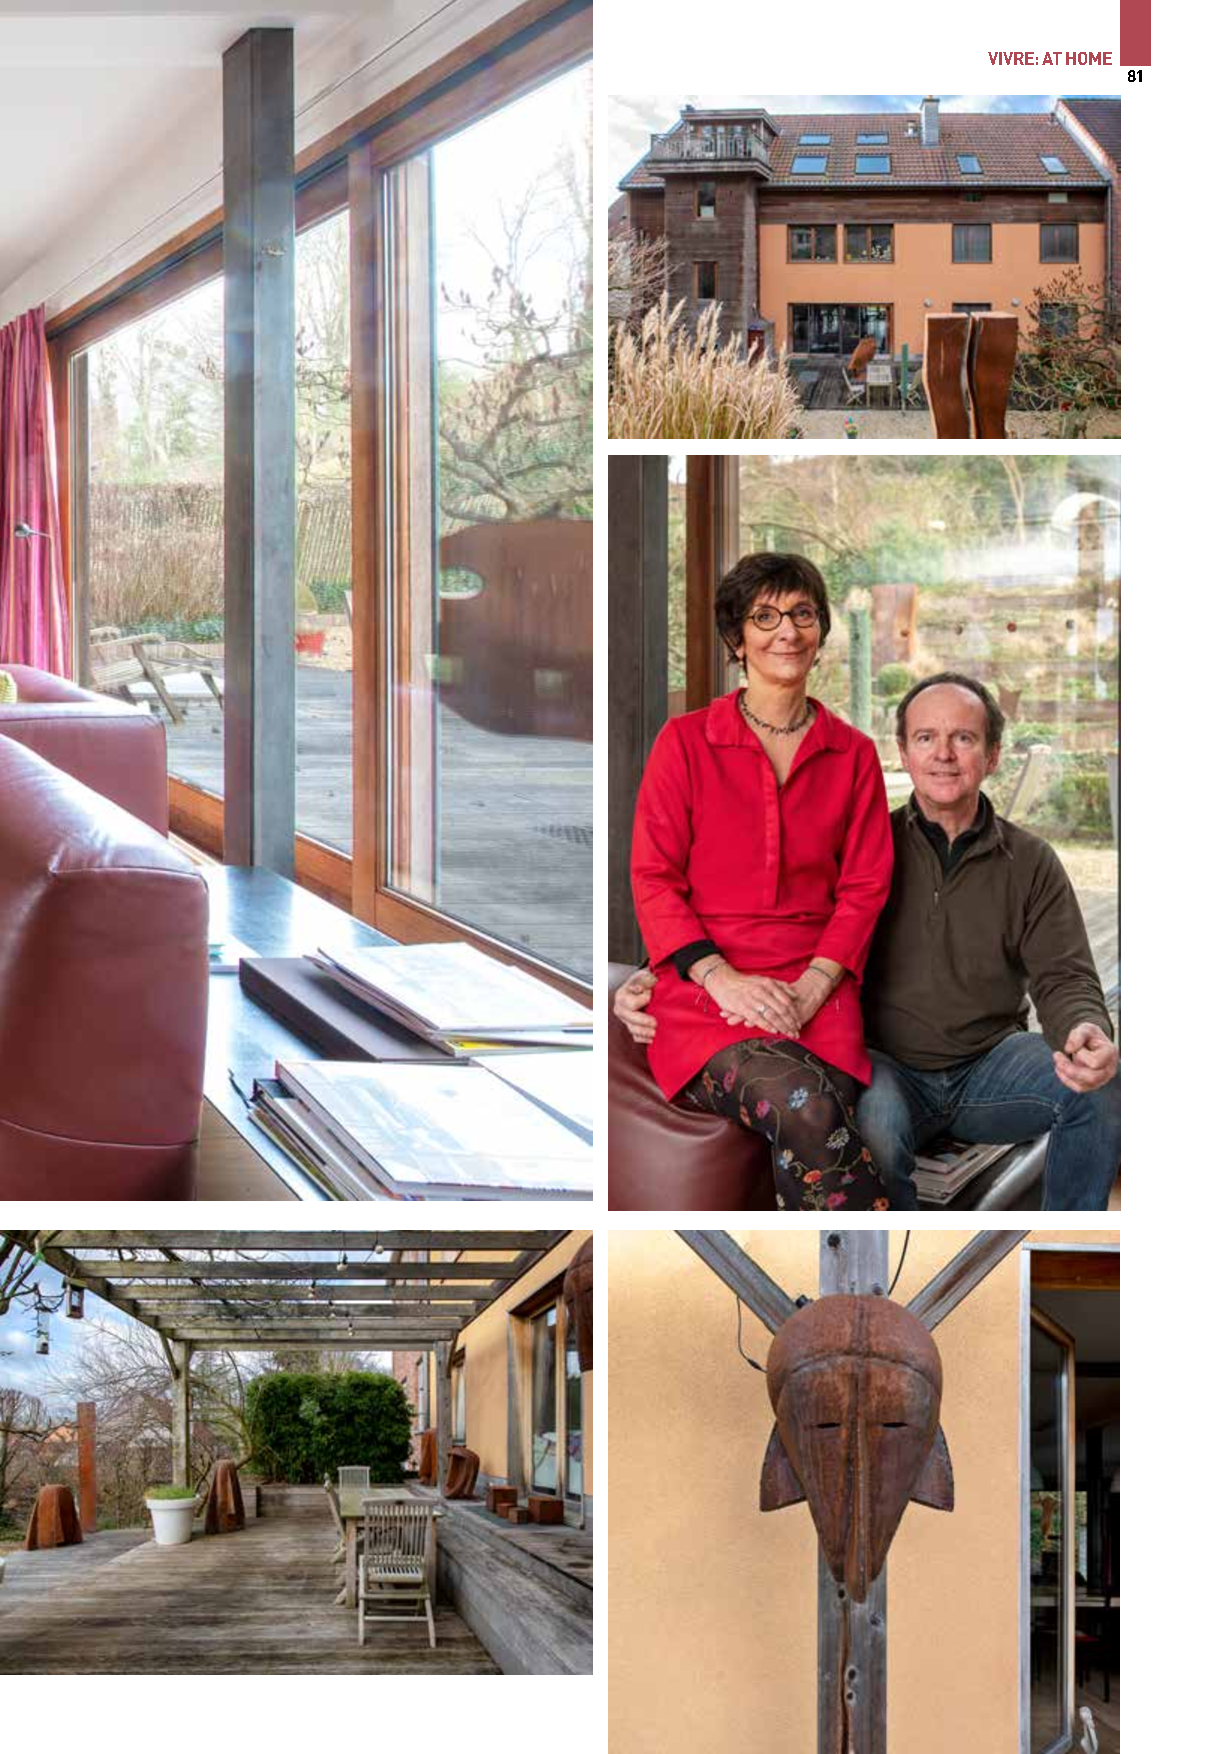
\includepdf[scale=0.95, nup=1x2, pages=1-2, angle=90]{maison1.pdf}
\end{landscape}
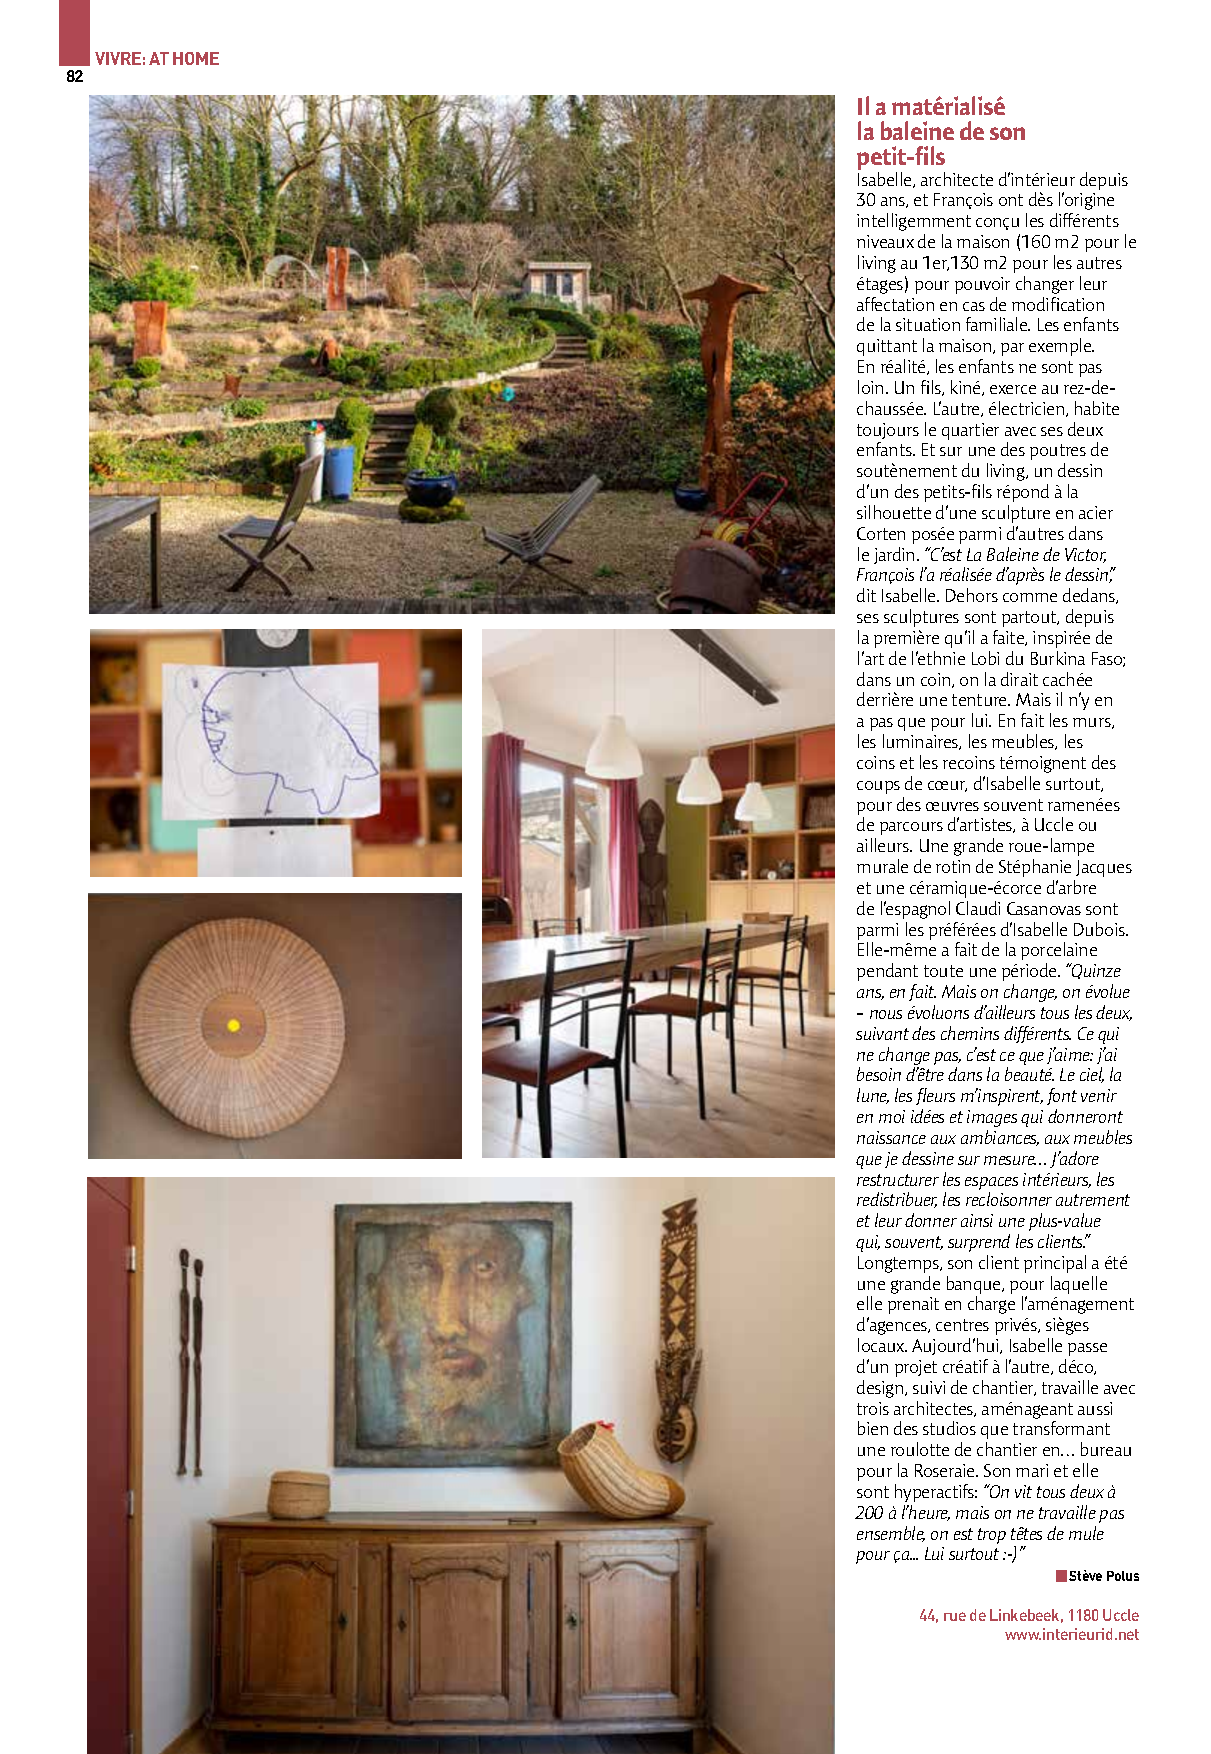
\includepdf[scale=0.95]{maison2.pdf}

\section{Courbe synthétique}
\label{appendix:b}

 \begin{center}

\begin{tikzpicture}

\begin{axis}[
date coordinates in=x,
enlarge x limits=false,
xmin=2014-01-01,
xmax=2019-12-31,
ymin=-20,
ymax=10,
xtick={2014-01-01, 2015-01-01, 2016-01-01, 2017-01-01, 2018-01-01, 2019-01-01},
xmajorgrids,
ytick={-20, -10, 0, 10},
title={Courbe synthétique globale du secteur de la construction en Belgique},
height=8cm,width=\linewidth,
enlarge x limits=false,
ylabel={Indice conjucturel},
legend entries={Séries dessaisonalisées et lissées, Séries brutes},
legend style={at={(0.5,-0.15)},anchor=north},
legend plot pos=left, legend columns=2,
x tick label style={at={(0.5,0)}},
xticklabel={~~~~~~~~~~~~~~~~\year}
]

\addplot[mark=none, smooth,draw=blue, ultra thick]
table[x index=0,y index=1, /pgf/number format/read comma as period]{Default.txt};
\addplot[mark=*, draw=black, thin]
table[x index=0,y index=1]{RAdonneesnonlissees.txt};

\end{axis}

\end{tikzpicture}

\end{center}

\section{Article sculpture François Canart}
\label{appendix:c}

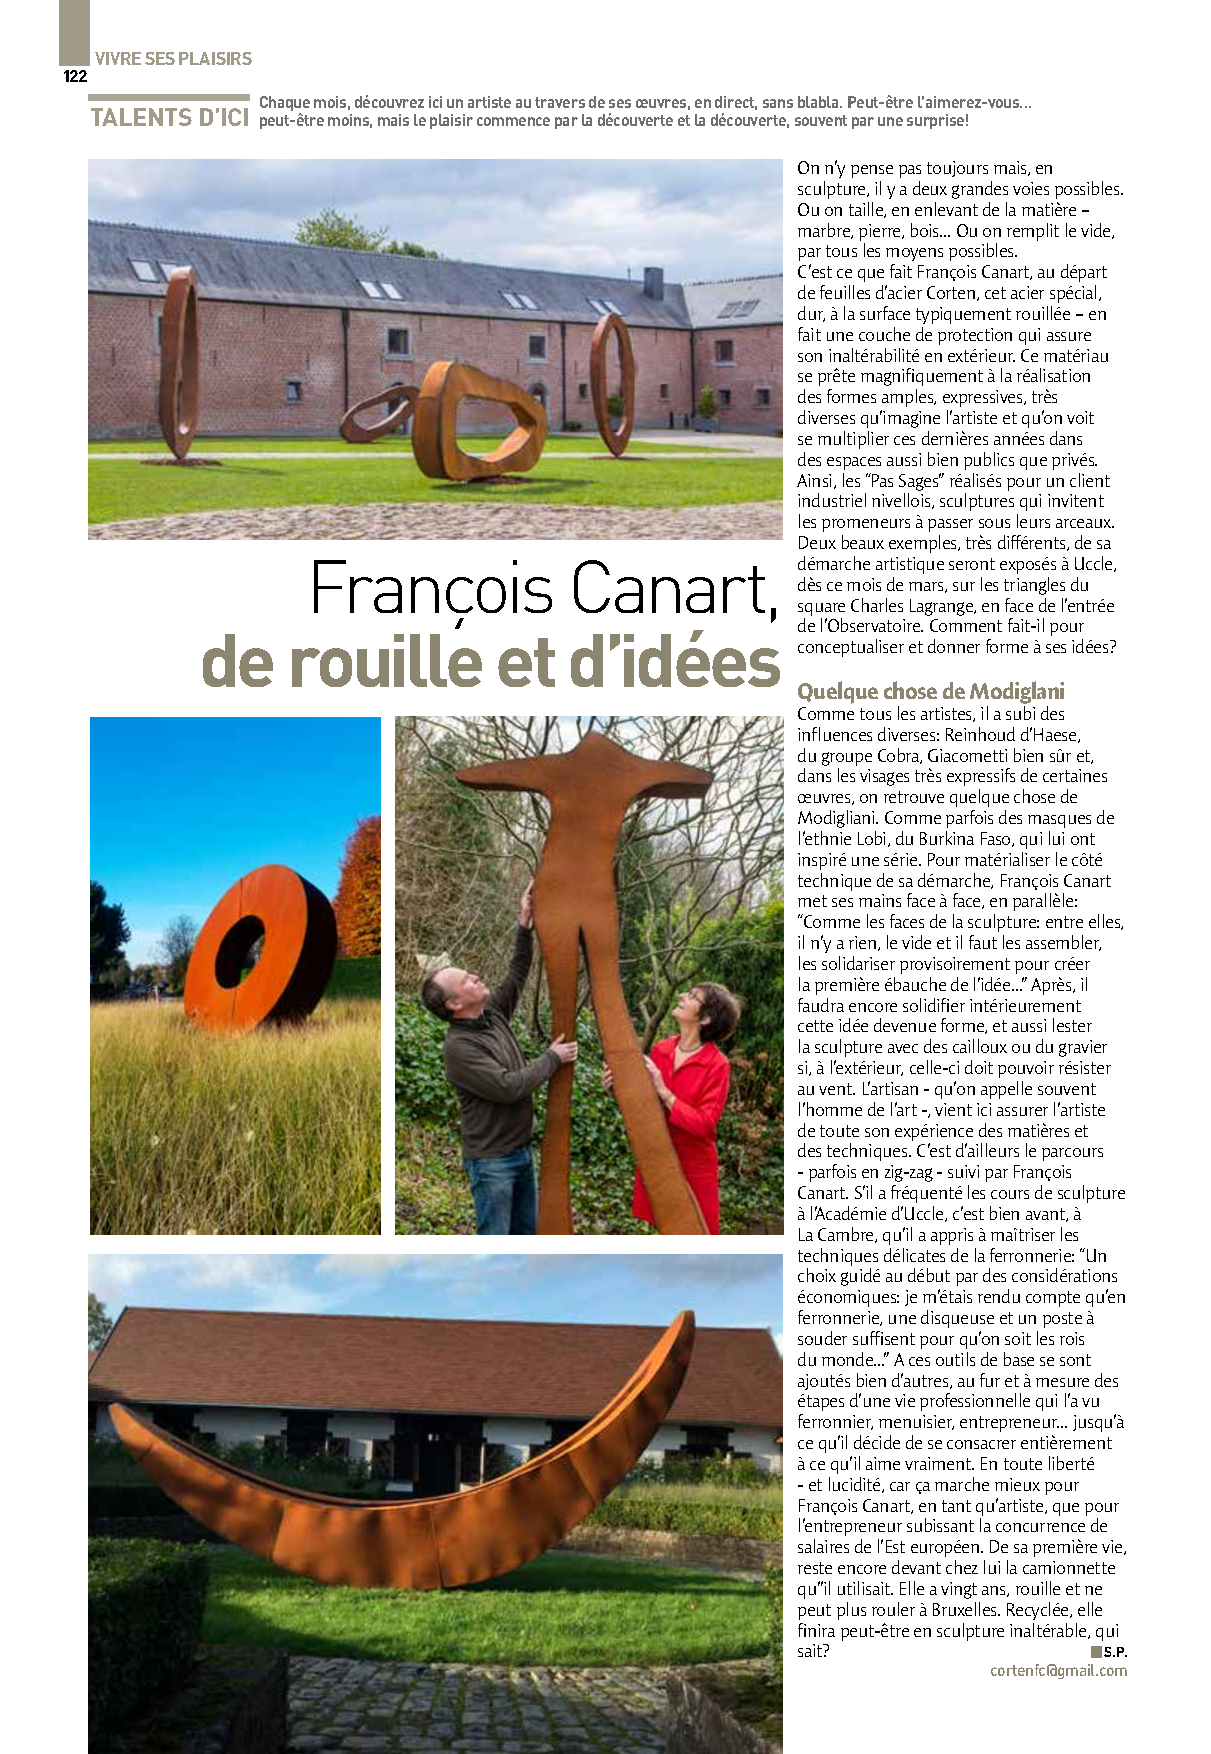
\includepdf[scale=0.95]{sculpture.pdf}

\section{Aperçu de l'interface de programmation}
\label{appendix:d}

\begin{landscape}
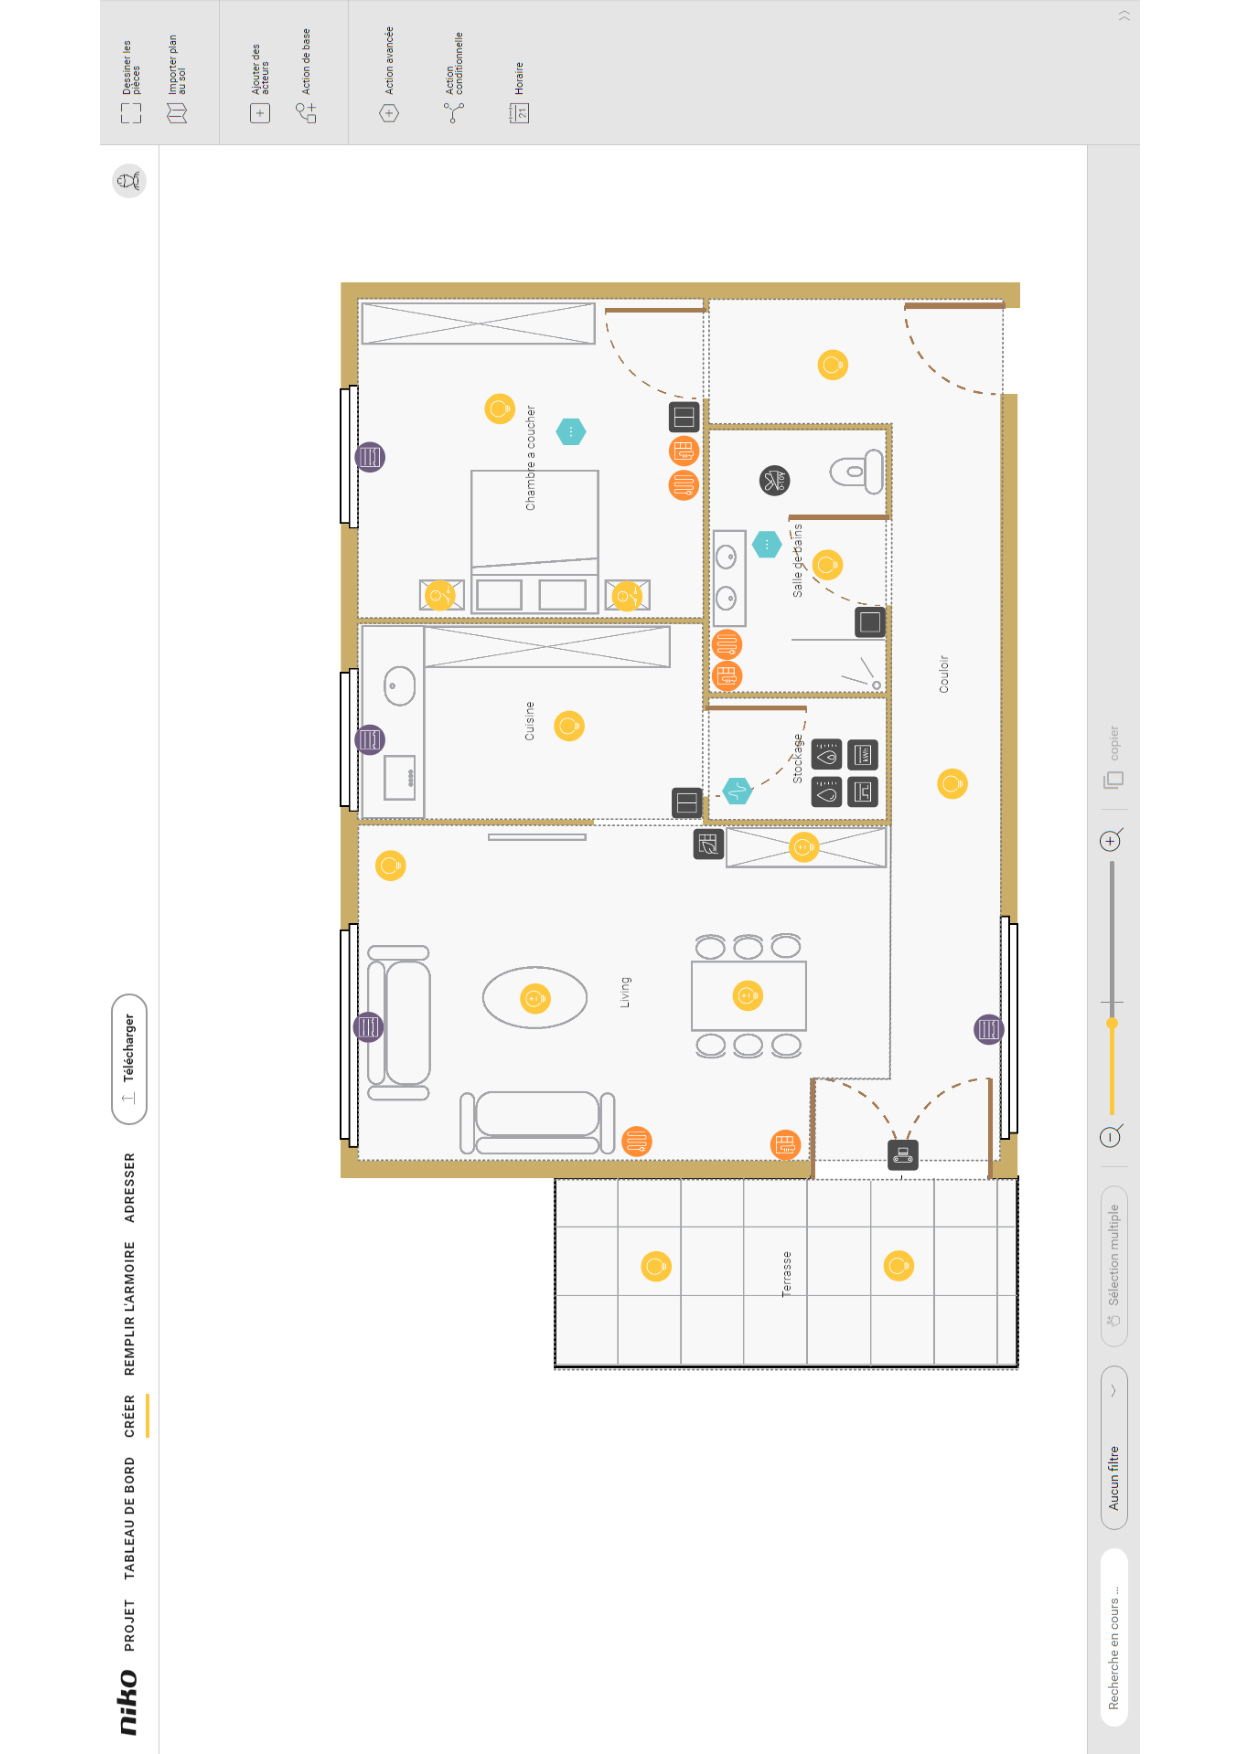
\includepdf[scale=0.95]{exempleNHC.pdf}
\end{landscape}

\section{Plan de l'installation électrique}
\label{appendix:e}

\begin{landscape}
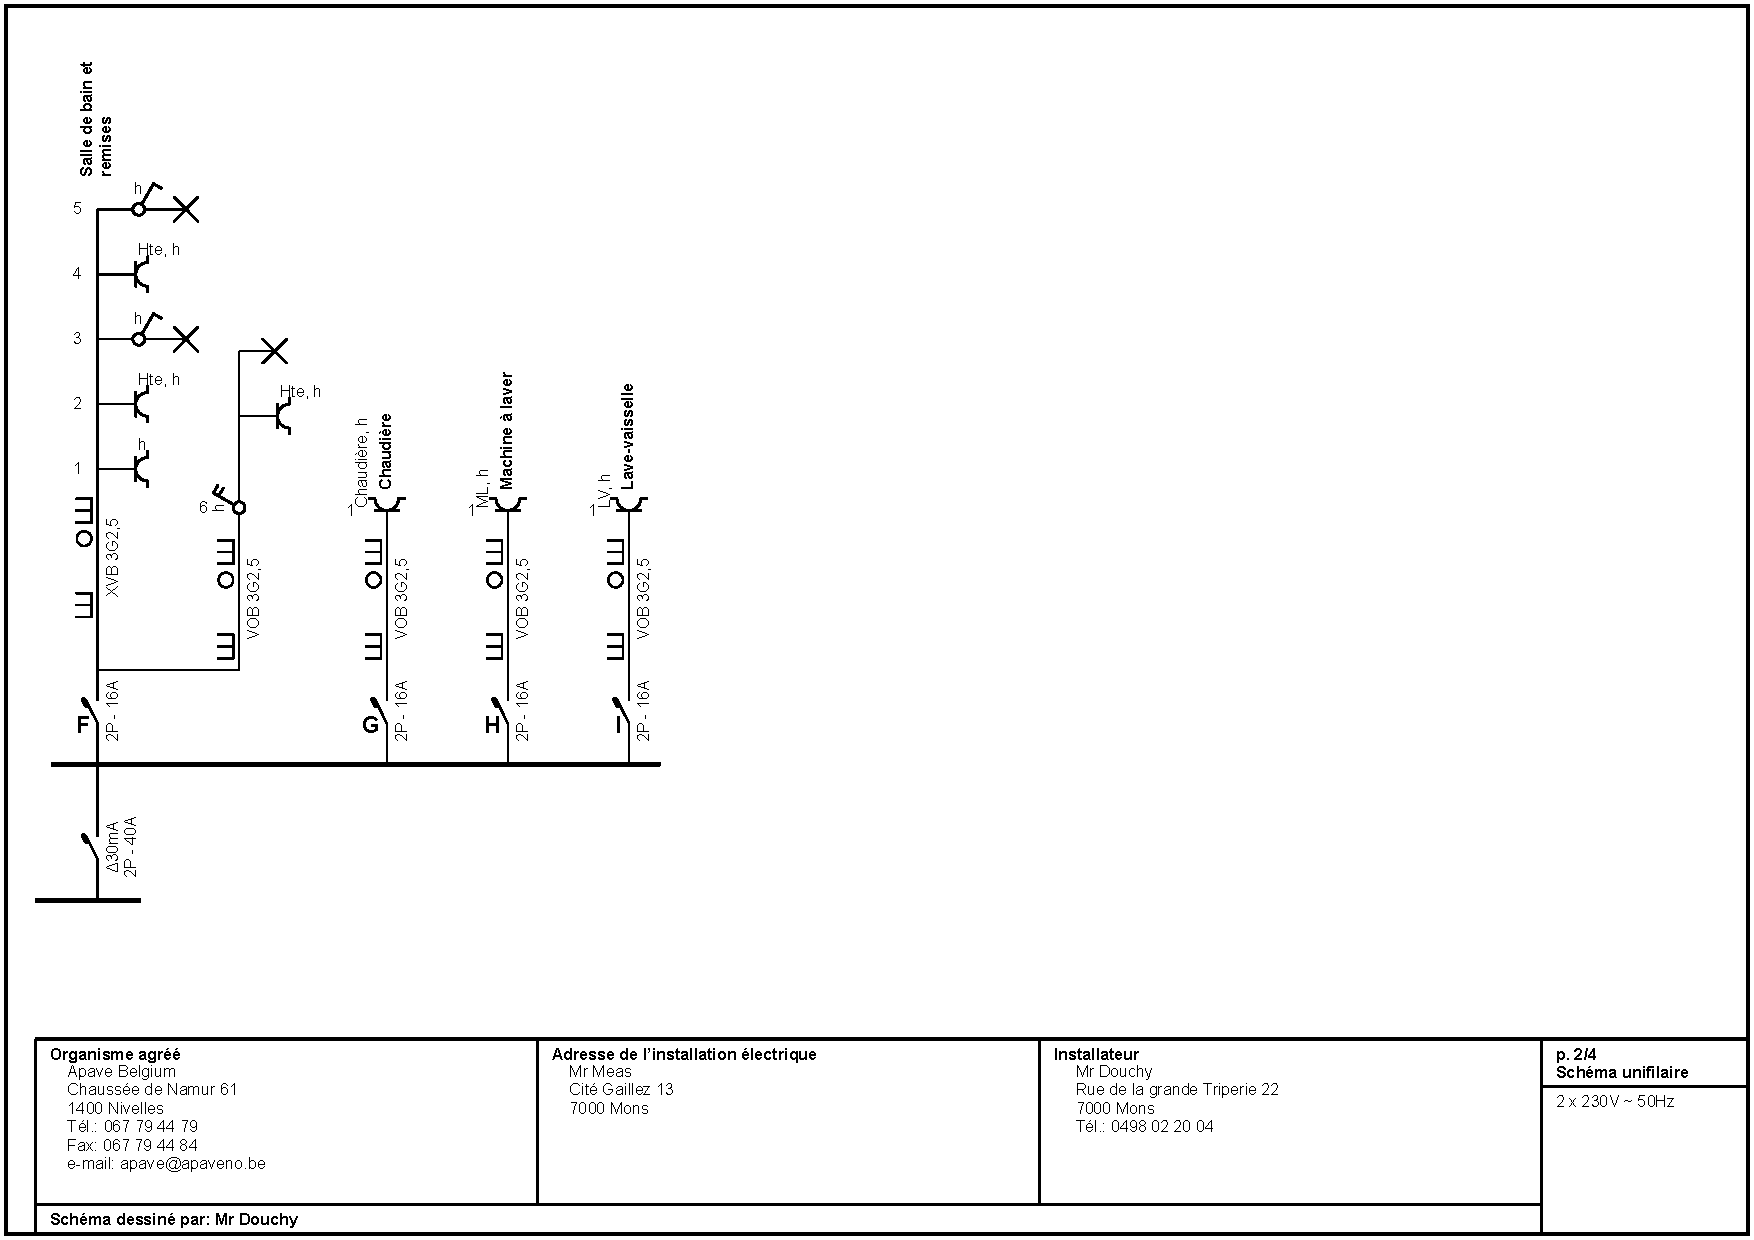
\includepdf[scale=0.95, nup=2x2, pages=1-4, angle=90]{Meas.pdf}
\end{landscape}

\end{appendix}

\end{document}
